
\documentclass{beamer}
\usetheme{ucl}

\usepackage[utf8]{inputenc}


%%% Increase the height of the banner: the argument is a scale factor >=1.0
%\setbeamertemplate{banner}[ucl][10.0]

%%% Change the colour of the main banner
%%% The background should be one of the UCL colours (except pink or white):
%%%   black,darkpurple,darkred,darkblue,darkgreen,darkbrown,richred,midred,
%%%   navyblue,midgreen,darkgrey,orange,brightblue,brightgreen,lightgrey,
%%%   lightpurple,yellow,lightblue,lightgreen,stone
\setbeamercolor{banner}{bg=darkpurple}
%\setbeamercolor{banner}{bg=yellow,fg=black}

%%% Add a stripe behind the banner
%\setbeamercolor{banner stripe}{bg=darkpurple,fg=black}

%%% The main structural elements
\setbeamercolor{structure}{fg=black}

%%% Author/Title/Date and slide number in the footline
\setbeamertemplate{footline}[author title date]

%%% Puts the section/subsection in the headline
% \setbeamertemplate{headline}[section]

%%% Puts a navigation bar on top of the banner
%%% For this to work correctly, the each \section command needs to be
%%% followed by a \subsection. Requires one extra compile.
% \setbeamertemplate{headline}[miniframes]
%%% Accepts an optional argument determining the width
% \setbeamertemplate{headline}[miniframes][0.3\paperwidth]


%%% Puts the frame title in the banner
%%% Won't work correctly with the above headline templates
%\useoutertheme{ucltitlebanner}
%%% Similar to above, but smaller (and puts subtitle on same line as title)
\useoutertheme[small]{ucltitlebanner}

%%% Gives block elements (theorems, examples) a border
% \useinnertheme{blockborder}
%%% Sets the body of block elements to be clear
% \setbeamercolor{block body}{bg=white,fg=black}

%%% Include CSML logo on title slide
%\titlegraphic{\includegraphics[width=0.16\paperwidth]{csml_logo}}

%%% Include CSML logo in bottom right corner of all slides
%\logo{\includegraphics[width=0.12\paperwidth]{csml_logo}}

%%% Set a background colour
% \setbeamercolor{background canvas}{bg=lightgrey}

%%% Set a background image
%%% Some sample images are available from the UCL image store:
%%%   https://www.imagestore.ucl.ac.uk/home/start
% \setbeamertemplate{background canvas}{%
%   \includegraphics[width=\paperwidth]{imagename}}



%%%%%% Some other settings that can make things look nicer
%%% Set a smaller indent for description environment
\setbeamersize{description width=2em}
%%% Remove nav symbols (and shift any logo down to corner)
\setbeamertemplate{navigation symbols}{\vspace{-2ex}}








\DeclareMathOperator{\Cov}{Cov}
\DeclareMathOperator{\Var}{Var}
\DeclareMathOperator{\E}{\mathbb{E}}
\DeclareMathOperator{\Proba}{\mathbb{P}}

\newcommand{\Covb}[2]{\ensuremath{\Cov\!\left[#1,#2\right]}}
\newcommand{\Eb}[1]{\ensuremath{\E\!\left[#1\right]}}
\newcommand{\Pb}[1]{\ensuremath{\Proba\!\left[#1\right]}}
\newcommand{\Varb}[1]{\ensuremath{\Var\!\left[#1\right]}}

% norm
\newcommand{\norm}[1]{\| #1 \|}

\newcommand{\indep}{\rotatebox[origin=c]{90}{$\models$}}





\usepackage{mathptmx,amsmath,amssymb,graphicx,bibentry,bbm,ragged2e}
\usepackage[english]{babel}

\makeatletter

\newcommand{\noun}[1]{\textsc{#1}}
\newcommand{\jitem}[1]{\item \begin{justify} #1 \end{justify} \vfill{}}
\newcommand{\sframe}[2]{\frame{\frametitle{#1} #2}}

\newenvironment{centercolumns}{\begin{columns}[c]}{\end{columns}}
%\newenvironment{jitem}{\begin{justify}\begin{itemize}}{\end{itemize}\end{justify}}



%\usetheme{Warsaw}
%\setbeamertemplate{footline}[text line]{}
%\setbeamertemplate{headline}{}
%\setbeamercolor{structure}{fg=purple!50!blue, bg=purple!50!blue}

%\setbeamersize{text margin left=15pt,text margin right=15pt}

%\setbeamercovered{transparent}


\@ifundefined{showcaptionsetup}{}{%
 \PassOptionsToPackage{caption=false}{subfig}}
\usepackage{subfig}

\usepackage[utf8]{inputenc}
\usepackage[T1]{fontenc}

\usepackage{multirow}


\makeatother

\def \draft {1}

\usepackage{xparse}
\usepackage{ifthen}
\DeclareDocumentCommand{\comment}{m o o o o}
{\ifthenelse{\draft=1}{
    \textcolor{red}{\textbf{C : }#1}
    \IfValueT{#2}{\textcolor{blue}{\textbf{A1 : }#2}}
    \IfValueT{#3}{\textcolor{ForestGreen}{\textbf{A2 : }#3}}
    \IfValueT{#4}{\textcolor{red!50!blue}{\textbf{A3 : }#4}}
    \IfValueT{#5}{\textcolor{Aquamarine}{\textbf{A4 : }#5}}
 }{}
}
\newcommand{\todo}[1]{
\ifthenelse{\draft=1}{\textcolor{red!50!blue}{\textbf{TODO : \textit{#1}}}}{}
}




\begin{document}

\title
[Exploration of an interdisciplinary scientific landscape]{Exploration of an interdisciplinary scientific landscape}
\author[Raimbault]{J.~Raimbault$^{1,2,3}$\\\medskip
$^{\ast}$\texttt{juste.raimbault@polytechnique.edu}
}

\institute[UCL]{$^{1}$Center for Advanced Spatial Analysis, University College London\\
$^{2}$UPS CNRS 3611 Complex Systems Institute Paris\\
$^{3}$UMR CNRS 8504 G{\'e}ographie-cit{\'e}s
}




\date[27/10/2020]{MLIS 2020\\
Machine Learning II\\
October 27th, 2020
}

\frame{\maketitle}


% Patterns of interdisciplinarity in science can be quantified through complementary dimen- sions. This paper studies as a case study the scientific environment of a generalist journal in Geography, Cybergeo, in order to introduce a novel methodology combining citation network analysis and semantic analysis. We collect a large corpus of around 200,000 arti- cles with their abstracts and the corresponding citation network that provides a first citation classification. Relevant keywords are extracted for each article through text-mining, allow- ing us to construct a semantic classification. We study the qualitative patterns of relations between endogenous disciplines within each classification, and finally show the comple- mentarity of classifications and of their associated interdisciplinarity measures. The tools we develop accordingly are open and reusable for similar large scale studies of scientific environments. Our contribution therefore provides, besides the methodology, a new way to construct open databases and study journals for which data are difficult to obtain.
% Citation network · Semantic network · Interdisciplinarity · Geography

\section{Introduction}


\sframe{Interdisciplinarity}{

% The development of interdisciplinary approaches is increasingly necessary for most of disciplines, both for further knowledge discovery but also societal impact of discover- ies, as it was for example recently coined by the special issue of Nature (2015). Inter- disciplinary research has furthermore a higher citation impact as shown by Chen et al. (2015), but traditional research institutions such as the Nobel price still fail to foster interdisciplinarity (Szell et al. 2018). Banos (2013) suggests that the development of such approaches must occur within a subtle spiral between and inside disciplines. An other way to interpret this phenomenon is to read it as the emergence of vertically inte- grated fields conjointly with horizontal questions as detailed in the Complex Systems roadmap (Bourgine et al. 2009). There are naturally multiple views on what exactly interdisciplinarity is and it actually depends on the domains involved: recent hybrid disciplines (see e.g. the ones exhibited by Bais (2010) such as astro-biology) are a good illustration of the case where entanglement is strong and new discoveries are vertically deep, whereas more loose fields such as “urbanism”, which have no precise definition and where integration is by essence horizontal, is an example of how transversal knowl- edge can be produced. Interactions between disciplines are not always smooth, as shows the misunderstandings when urban issues were recently introduced to physicists as Dupuy and Benguigui (2015) recalls.

\justify

\textit{Importance of interdisciplinary approaches for knowledge itself but also to solve complex issues such as global change and sustainability}

\bigskip

$\rightarrow$ different types of integration between disciplines in theory 

\cite{chavalarias2009french} and in practice \cite{dupuy2015sciences}

\bigskip
\bigskip

\centering


\includegraphics[width=0.49\textwidth]{figures/erc.png}\hspace{0.5cm}

\includegraphics[width=0.45\textwidth]{figures/miti.png}


}

\sframe{Quantitative Studies of Science}{

% These concerns are part of an understanding of processes of knowledge production in which evidence-based perspectives, involving quantitative approaches, play an impor- tant role. These paradigms can be understood as a quantitative epistemology follow- ing Chavalarias and Cointet (2013). Quantitative measures of interdisciplinarity would therefore be part of a multidimensional approach of the study of science that is in a way “beyond bibliometrics” (Cronin and Sugimoto 2014). The focus of this paper is posi- tioned within this stream of research. The possible methods for quantitative insights into epistemology are numerous. A good illustration of the variety of approaches is given by network analysis. Using citation network features, a good predicting power for citation patterns is for example obtained by Newman (2014). The visualisation of citation networks can help to identify qualitative changes in the structure of disciplines (Chen 2004). Visual analytics indeed play a crucial role in the study of knowledge (Börner et al. 2003). Co-authorship networks can also be used for predictive models (Sarigöl et al. 2014). Disciplines can be stratified into layers to reveal communities between them and therein collaboration patterns (Battiston et al. 2015). Networks analysis are used in other fields such as economics of innovation: for example, Choi and Hwang (2014) propose a method to identify technological opportunities by detecting important keywords from the point of view of topological measures. In political science, Gaumont et al. (2018) use the gargantext platform to offer a clear view of political debates seen from the proxy of twitter. Such works allow to understand the dynamics of knowledge. For example, Shibata et al. (2008) use topological analysis of the citation network to detect emerging research fronts. Citation and co-citations patterns are at the basis of the generic framework devel- oped by Chen (2006) to detect emerging trends in science. The case of Nanoscience is studied by Bonaccorsi and Vargas (2010) as a case of an emerging field exhibiting pro- liferating patterns for the keywords used. Large scale initiatives to map science, such as the UCSD map of science (Börner et al. 2012), are crucial both for the understanding of scientific environments, for scien- tific policies, and for social and technological transfers. Leydesdorff and Rafols (2009) describe a global map with nested discipline maps. An other important quantitative insight into science is the modeling of its dynamics (Börner et al. 2011; Scharnhorst et al. 2012), aimed at understanding processes through which collective scientific intelligence and its structures do emerge. This can include the modeling of social processes (Edmonds et al. 2011), of research institutions (Rouse et al. 2018), or of the dynamics of competing theories themselves (Akerlof and Michaillat 2018). We now review with more details the different approaches to define and measure interdisciplinarity.

Quantitative Studies of Science beyond bibliometrics \cite{cronin2014beyond}:

\medskip

\begin{itemize}
	\item Maps of science \cite{borner2012design}\cite{leydesdorff2009global}
	\item Modeling science dynamics \cite{borner2011modeling}
	\item Modeling social processes in science \cite{edmonds2011simulating}
	\item Citation \cite{shibata2008detecting}, co-authorship, semantic networks \cite{gaumont2017methods}
	\item Quantitative epistemology \cite{chavalarias2013phylomemetic}
\end{itemize}


}


\sframe{Defining and measuring interdisciplinarity}{

% Definitions of interdisciplinarity itself and indicators to measure it have already been tackled by a large body of literature. Huutoniemi et al. (2010) recall the difference between multidisciplinary (an aggregate of works from different disciplines) and inter- disciplinary (implying a certain level of integration) approaches. They construct a qual- itative framework to classify types of interdisciplinarity, and for example distinguish empirical, theoretical and methodological interdisciplinarities.Wagner et al. (2011) find that knowledge integration is crucial for interdisciplinarity, and that it can occur at different levels, from the single scientist to the research team or the field. Hall et al. (2008) confirm the role of the social aspect in potential interdiscipli- nary collaborations, by proposing to include the readiness to collaborate in the evalua- tion of corresponding research units. The multidimensionnal aspect of interdisciplinar- ity is confirmed even within a specific field such as literature (Austin et al. 1996). Beside these different conceptual approaches to interdisciplinarity, there exist several methodological means to measure it, of which we now give an overview. A first way to quantify interdisciplinarity of a set of publications is to look at the proportion of disciplines outside a main discipline in which they are published, as Rinia et al. (2002) do for the evaluation of projects in physics, complementary with judgement of experts. Porter et al. (2007) designate this measure as specialization, and compare it with a measure of integration, also called the Rao-Stirling index, which is given by the spread of citations done by a paper within the different Subject Categories (classification of the Web of Knowledge). Larivière and Gingras (2010) use it on a Web of Science corpus to show the existence of an optimal intermediate level of interdisciplinarity for the cita- tion impact within a five year window. A similar work is done in Larivière and Gingras (2014), focusing on the evolution of measures on a long time range. The influence of missing data on this index is studied by Moreno et al. (2016), providing an extended framework taking into account uncertainty. Other indices based on citation practices have been introduced, such as by Rod- ríguez (2017) which proposes an entropy-based index to classify the behavior of journal regarding knowledge import or export. Zhang et al. (2016) recall mathematical proper- ties that need to be verified by diversity indices (such as symmetry or scale-invariance), and proposes that Hill-type indices are more relevant than entropy. Mugabushaka et al. (2016) show that most of existing indices are a particular cases of Leinster-Cobbold diversity indices, which correspond to a third generation of indices to measure diversity in ecology. Leydesdorff and Rafols (2011) compare different indi- ces at the level of journals, and show that they appear to capture different dimensions of this phenomenon in a complementary way. The use of bottom-up network measures has also been proposed to quantify inter- disciplinary research: Porter and Rafols (2009) combine the integration index with a mapping technique which consists in visualisation of synthetic networks constructed by co-citations between disciplines. Leydesdorff (2007) shows that the betweenness centrality is a relevant indicator of interdisciplinarity, when considering appropriate citation neighborhood. A multilayer network approach was proposed in Omodei et al. (2017), using bipartite networks of papers and scholars, in order to produce measures of interdisciplinarity using generalized centrality measures. Rafols and Meyer (2009) combine diversity indices with measures of network coherence, which capture the inte- gration of knowledge.
% Semantic analysis and interdisciplinarity
%A particular entry to the quantification of interdisciplinarity is semantic analysis of docu- ments. Nichols (2014) uses Latent Dirichlet Allocation topic modeling to characterize interdisciplinarity of awards in particular sciences. Palchykov et al. (2016) do the same for papers in physics based on concept extraction from full texts, and show that the endog- enous classes differ from the top-down subjects classification. Semantic networks are oth- erwise well studied in social sciences, such as for example Gurciullo et al. (2015) which analyze semantic networks of political debates. Bouveyron et al. (2018) introduce a block model for network clustering which includes textual information of nodes. Boyack et al. (2011) benchmark several text-based clustering methods. Semantic analysis can be coupled with other dimensions, and in particular citation net- work analysis. Brás et al. (2017) study oncology by coupling the semantic aspects with institutional aspects. Zhang et al. (2010) describe cross-journals citation clusters in terms of their semantic content, but do not produce an endogenous semantic classification. Gerow et al. (2018) find that the citation influence and the discursive influence of scholars are complementary dimensions of academic success, by using topic modeling for the semantic classification of their work.


\begin{itemize}
	\item Difference between multi- and interdisciplinary, and empirical, theoretical or methodological interdisciplinarity \cite{huutoniemi2010analyzing}
	\item Specialization indices (Rao-Stirling) \cite{lariviere2010relationship}
	\item Diversity indices (Leinster-Cobbold) \cite{mugabushaka2016bibliometric}
	\item Network-based indices \cite{leydesdorff2007betweenness} \cite{rafols2009diversity}
	\item Semantic aspects of interdisciplinarity \cite{nichols2014topic} \cite{bouveyron2016stochastic}	
\end{itemize}




}


\sframe{Proposed approach}{

% We develop in this paper a case study coupling citation network exploration and analysis with text-mining, aiming at mapping the scientific landscape in the neighborhood of a par- ticular journal. Our aim is twofold: (1) introduce a methodology coupling the two aspects; (2) introduce tools which allow the analysis of journals for which data is difficult to obtain, when e.g. not referenced in main databases. We study an electronic journal in Geography, namely Cybergeo,1 that publishes arti- cles within all subfields of Geography and is in that way multidisciplinary. The choice is initially due to data availability, but ensures several constraints making it highly relevant to the objectives given above. First of all, the “discipline” of Geography is very broad and by essence interdisciplinary (Bracken 2016): the spectrum ranges from Human and Criti- cal geography to physical geography and geomorphology, and interactions between these subfields are numerous. Secondly, bibliographical data is difficult to obtain, raising the concern of how the perception of a scientific landscape may be shaped by actors of the dis- semination and thus far from objective, and making technical solutions as the ones we will consequently develop here crucial tools for an open and neutral science. Finally it makes a particularly interesting case study as the editorial policy is generalist and concerned with open science issues such as peer-review ethics transparency (Wicherts 2016), open data and model practices, as recalled by Pumain (2015), and this work contributes to these by fostering the opening of reflexivity. Our approach combine semantic communities analysis with citation network to extract features such as interdisciplinarity measures. Our contribution is original regarding previ- ous works quantifying interdisciplinarity since it uses bottom-up community reconstruc- tion both in the citation and in the semantic dimension. Our work naturally differ from studies in which the classification mapped is exogenous, such as institutional thesaurus as mapped by Boyack (2017). Zhang et al. (2010) combine citation cluster with seman- tic analysis, but the semantic clusters are exogenous. We also differ from several previous work using endogenous semantic information, as Vugteveen et al. (2014) for example only use titles and combine them with references for the proximity measure, whereas we use more textual information with abstracts and a more refined method to extract keywords. Bouveyron et al. (2018) use both information simultaneously for the classification, captur- ing thus orthogonal dimensions with more difficulty. Our contribution is original and significant on at least two aspects: 1. We combine endogenous classifications in a network multilayer fashion; 2. A large dataset is constructed from scratch to study a journal not referenced in main databases, tackling both data retrieval and large scale data processing issues. Light et al. (2014) already introduced a large scale open database and associated tools for the study of science. Our work is complementary as our tool allow the retrieval of targeted data which may not be referenced in such databases. The rest of the paper is organized as follows: we describe in the next section the dataset used and the data collection procedure. We then study properties of the citation network and describe the procedure to construct the semantic classification through text-mining. We finally study complementary measures of interdisciplinarity obtained with the different classifications.

\textit{Difficulty to quantify interdisciplinarity (i) through multiple complementary dimensions; (ii) when data is not straightforward to gather.}

\bigskip

For a case study journal in Geography (Cybergeo, European Journal of Geography \url{https://journals.openedition.org/cybergeo/})

\medskip

$\rightarrow$ construct a database from heterogenous sources

\medskip

$\rightarrow$ quantify interdisciplinarity with citation and semantic networks

\bigskip

\centering

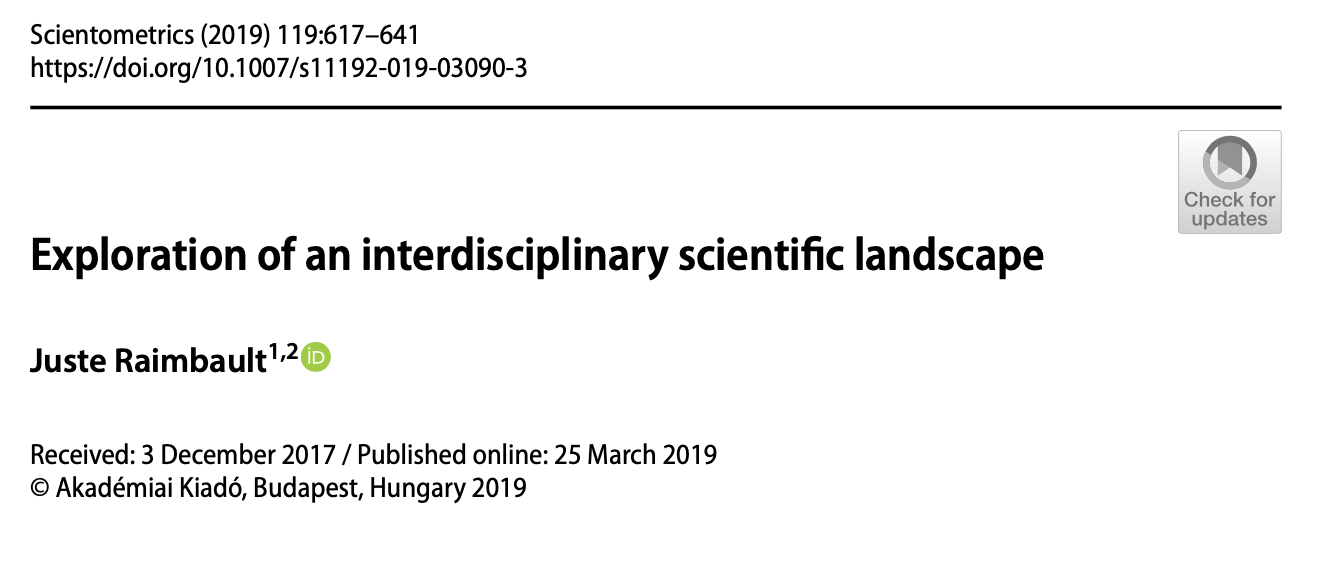
\includegraphics[width=0.9\textwidth]{figures/paper.png}


}

\section{Database construction}

\sframe{Data collection}{

% Our approach imposes some requirements on the dataset used, namely: (1) cover a certain neighborhood of the studied journal in the citation network in order to have a consistent view on the scientific landscape; (2) have at least a textual description for each node. For these to be met, we need to gather and compile data from heterogeneous sources. We use therefore an application specifically designed, which general architecture is given in Fig. 1. Source code of the application2 and all scripts used in this paper are available on the open git repository of the project. The data collection application is written in Java, natu- ral language processing in python, and network analyses in R using the igraph pack- age. Network visualisation are done with the Gephi software. Database used are MySql (production base of the journal) and MongoDB (semantic network construction). Raw and processed data are also openly available on Dataverse.3 We recall that an important con- tribution of this paper is the construction of such an hybrid dataset from heterogeneous sources, and the development of associated tools that can be reused and further developed for similar purposes.

Data collected from heterogenous sources: journal production database, google scholar for citation links, Mendeley for abstracts.

\medskip

Refactored open source java library for data collection: \url{https://github.com/JusteRaimbault/BiblioData}

\bigskip

\centering

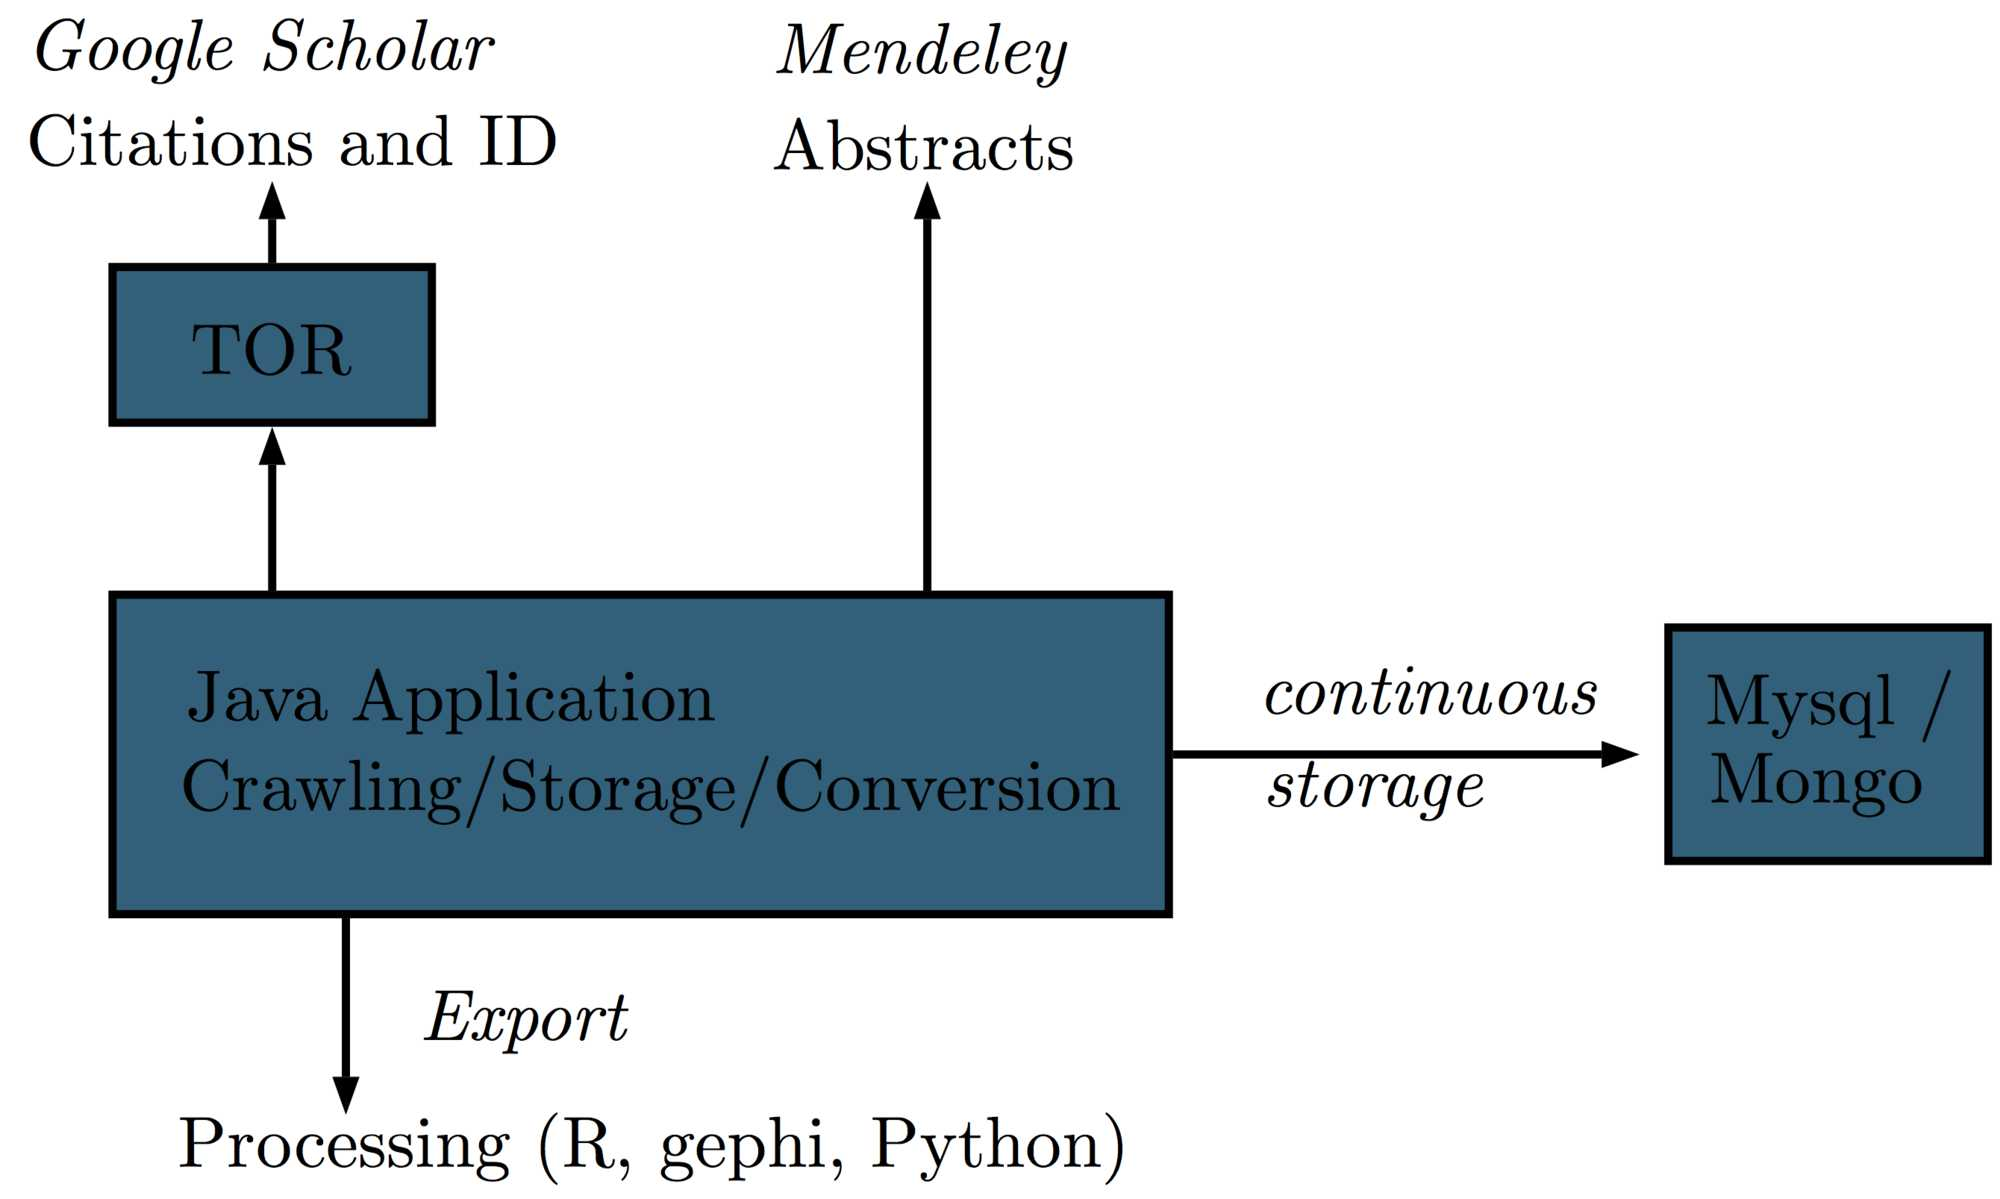
\includegraphics[width=0.7\textwidth]{figures/Fig1.jpg}

}

\sframe{Dataset}{

% % The production database of Cybergeo (snapshot taken in February 2016, provided by the editorial board), provides after pre-processing the initial database of articles, with basic information (title, abstract, publication year, authors). The processed version used is avail- able together with the full database constructed, as a mysql dump, at the address given above. This base provide also bibliographical records of articles that give all references cited by the initial base (forward citations for the initial corpus).
% Citation data is collected from Google Scholar, that is the only source for incoming citations (Noruzi 2005) in our case as the journal is poorly referenced in other databases.4 We are aware of the possible biaises using this single source (see e.g. Bohannon 2014),5 but these critics are more directed towards search results or possible targeted manipulations than the global structure of the citation network. The automatic collection requires the use of a crawling software to pipe requests, namely TorPool (Raimbault 2016) that provides a Java API allowing an easy integration into our application of data collection. A crawler can therethrough retrieve html pages and get backward citation data, i.e. all citing articles for a given initial article. We retrieve that way two sub-corpuses: references citing papers in Cybergeo and references citing the ones cited by Cybergeo. At this stage, the full corpus contains around 4 × 105 references. For the sake of simplicity, we will denote by reference any standard scientific produc- tion that can be cited by another (journal paper, book, book chapter, conference paper, communication, etc.) and contains basic fields (title, abstract, authors, publication year). We work in the following on networks of references, linked by citations.
% A textual description for all references is necessary for a complete semantic analysis. We use for this an other source of data, that is the online catalog of Mendeley reference manager software Mendeley (2015). It provides a free API allowing to get various records under a structured format. Although not complete, the catalog provides a reasonable cov- erage in our case, around 55% of the full citation network. This yields a final corpus with full abstracts of size 2.1 × 105. The structure and descriptive statistics of the corresponding citation network is recalled in Fig. 2.

Citation network with abstract coverage: $\simeq 2.1\cdot 10^5$ papers

\bigskip

\centering

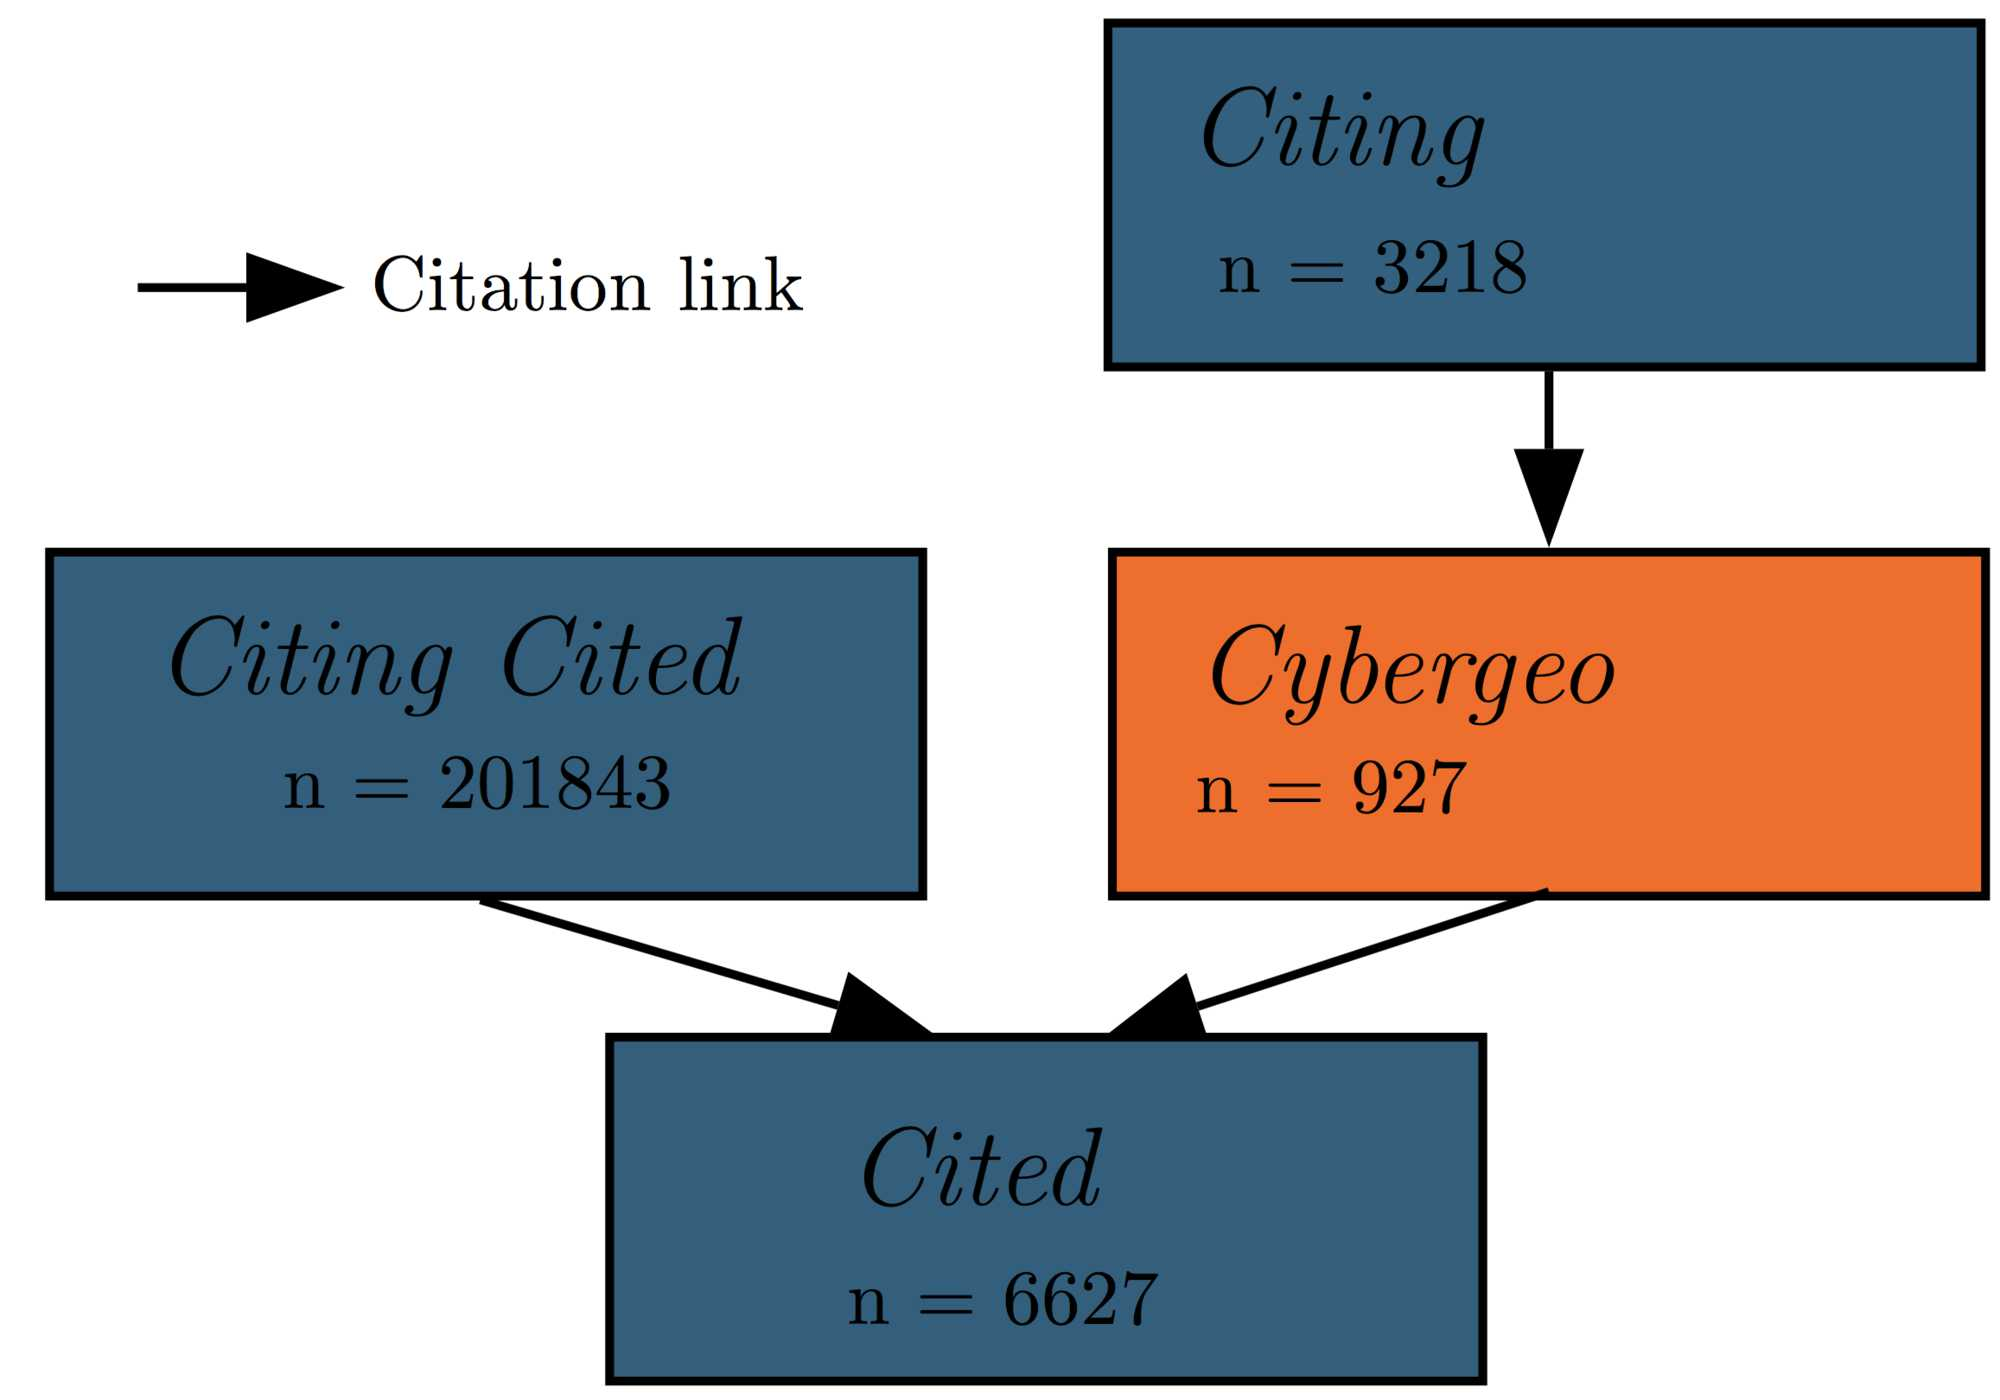
\includegraphics[width=0.7\linewidth]{figures/Fig2.jpg}

}


\section{Methods and results}


\sframe{Citation network properties}{

%As detailed above, we are able by the reconstruction of the citation network at depth ±1 from the original 927 references of the journal to retrieve around 45 × 106 references, on which 2.1 × 105 have an abstract text allowing semantic analysis. A first glance on cita- tion network properties provides useful insights. Average in-degree (which gives the cumu- lated number of citations since a reference was published) on references for which it can be defined has a value of d̄ = 121.6, whereas for articles in Cybergeo we have d̄ = 3.18. This difference suggests a variety for status of references, from old classical works (the most cited has 1051 incoming citations) to recent less influential works.
%This diversity is confirmed by the hierarchical organisation examined in Fig. 3 that unveils three superposed regimes. More precisely, we look at the rank-size plot, given by the logarithm of the number of citations received as a function of the rank of the paper. Scaling properties, which emerge in several models of network growth and are pervasive in real-world networks, are a powerful tool to understand the organisation of complex systems (Barabási and Albert 1999).
%We find, as expected (Redner 1998), localized power-law behaviors. A first set of around 150 references shows a very low hierarchy (rank-size exponent 𝛼 = 0.01) and corresponds to classical references in different disciplines. A second regime (𝛼 = 1.56) is much more hierarchized, followed by a last regime less hierarchical (𝛼 = 0.75) containing more recent papers (average publication year mid-2005, against mid-1998 for the second and 1983 for the first).

\centering

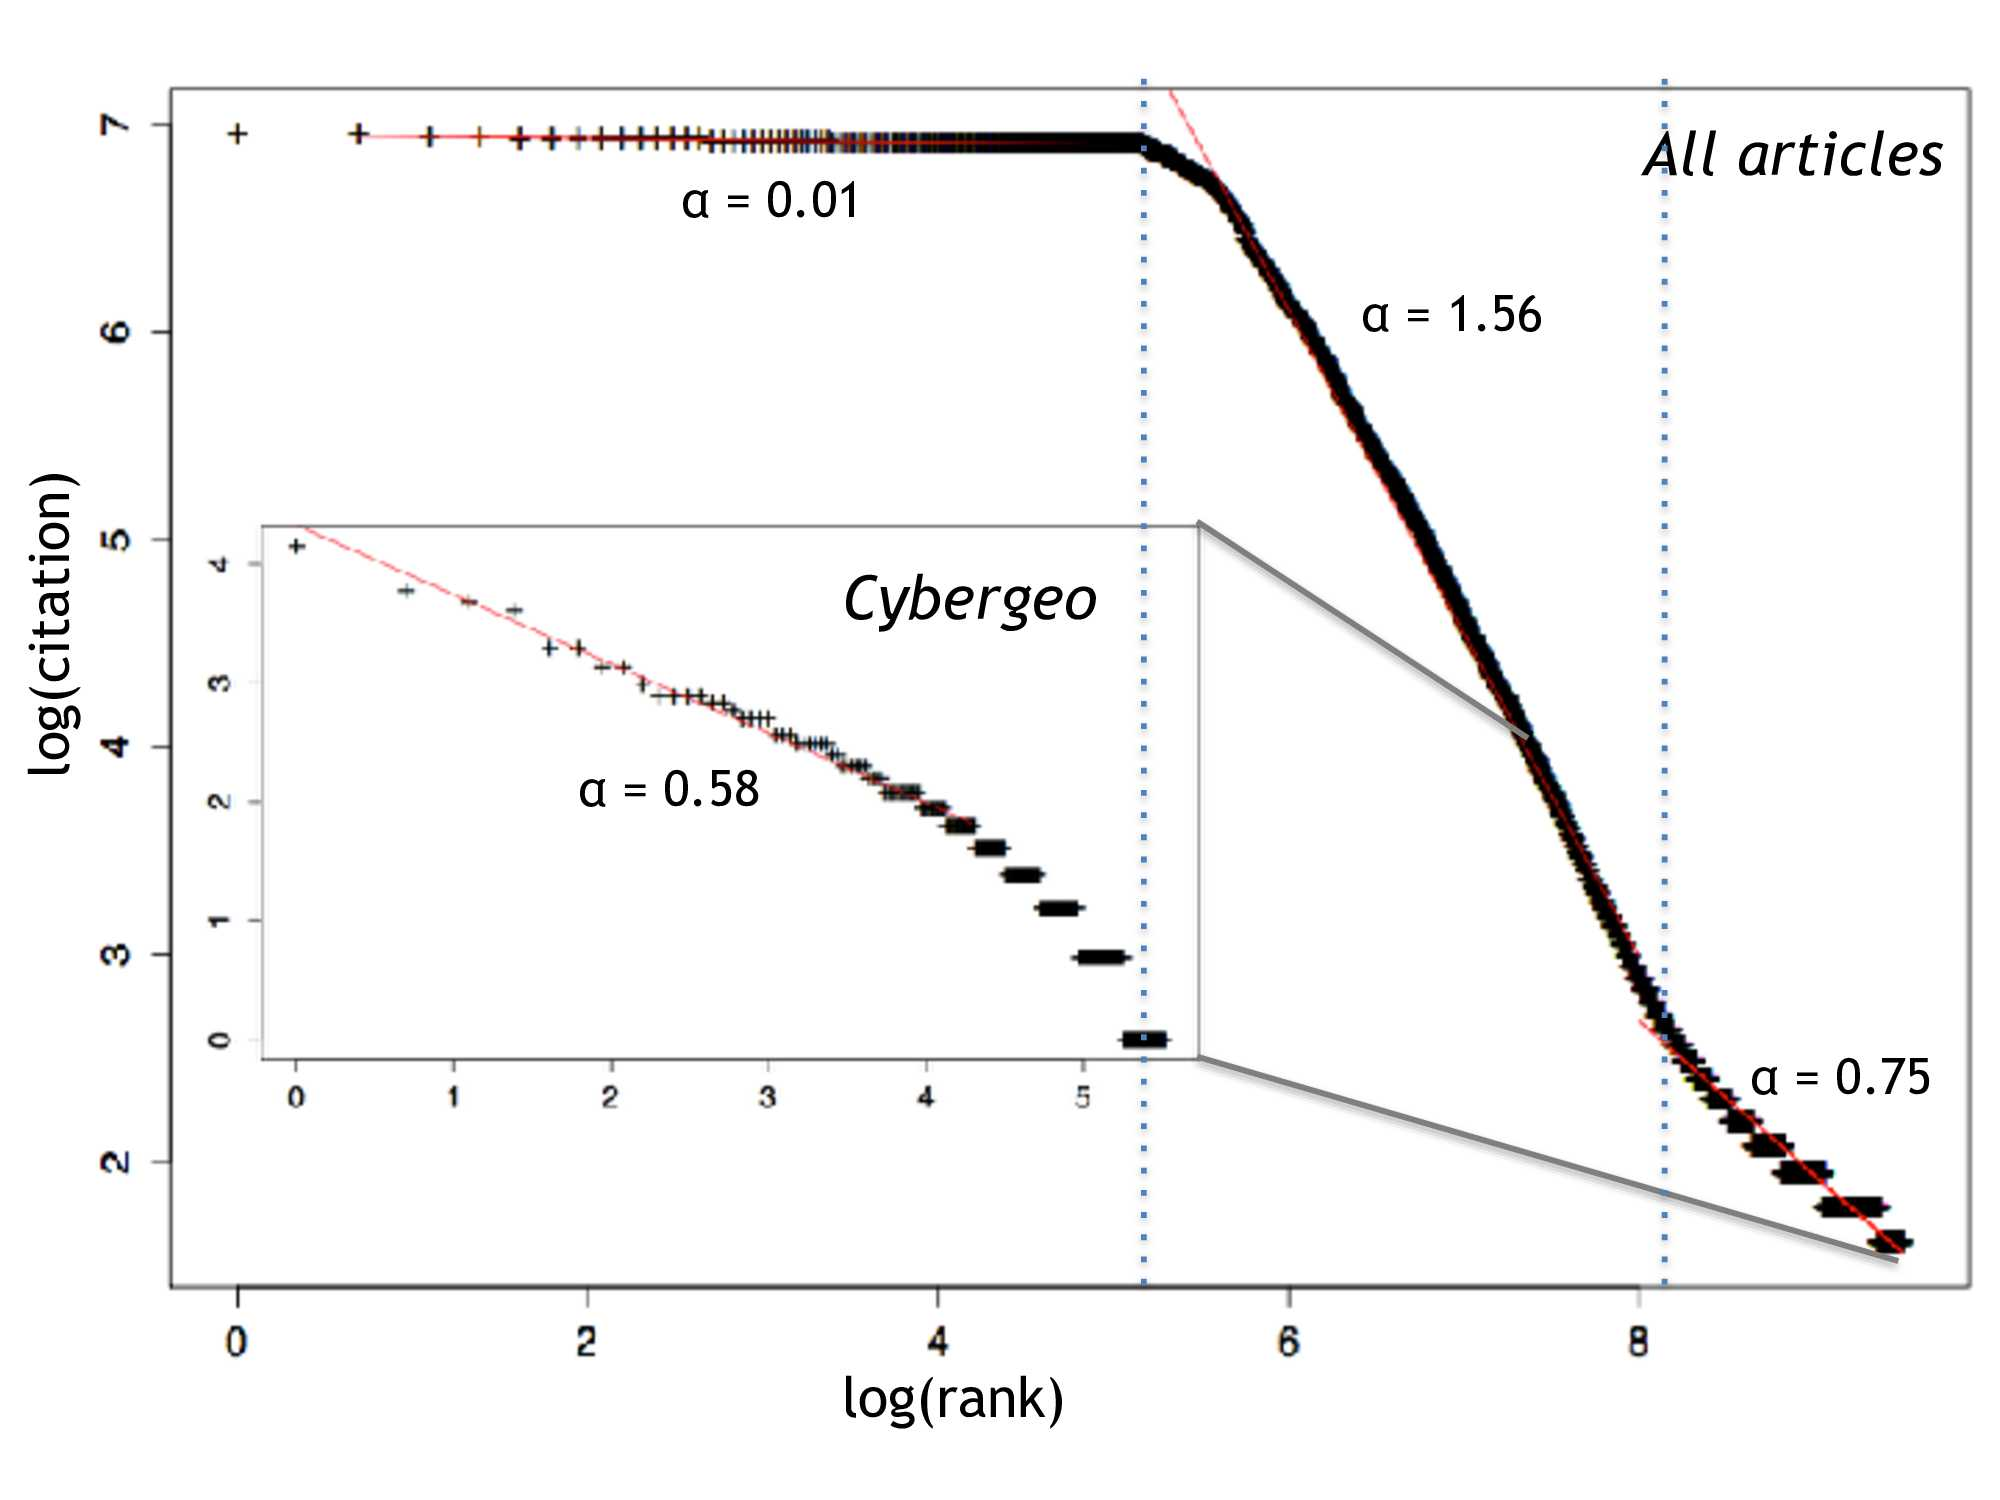
\includegraphics[width=0.9\textwidth]{figures/Fig3.jpg}

}

\sframe{Citation network properties}{

% Other topological properties reveal typical patterns of citation practices, as for example the existence of high-order cliques. Cliques are subset of nodes between which all pos- sible connections exist. Their existence implies citation practices in which all previous papers are systematically cited in new works. The compatibility of this process with the cumulative nature of knowledge may be questionable (Pumain 2005), since the previous knowledge production process is reconstructed each time instead on relying only on the most recent state of knowledge. An exemple of such a clique in shown in Fig. 4, where 6 publications studying the fractal nature of urban structures all cite the previous publica- tions in the clique.

\textit{Example of the largest citation clique}

\centering

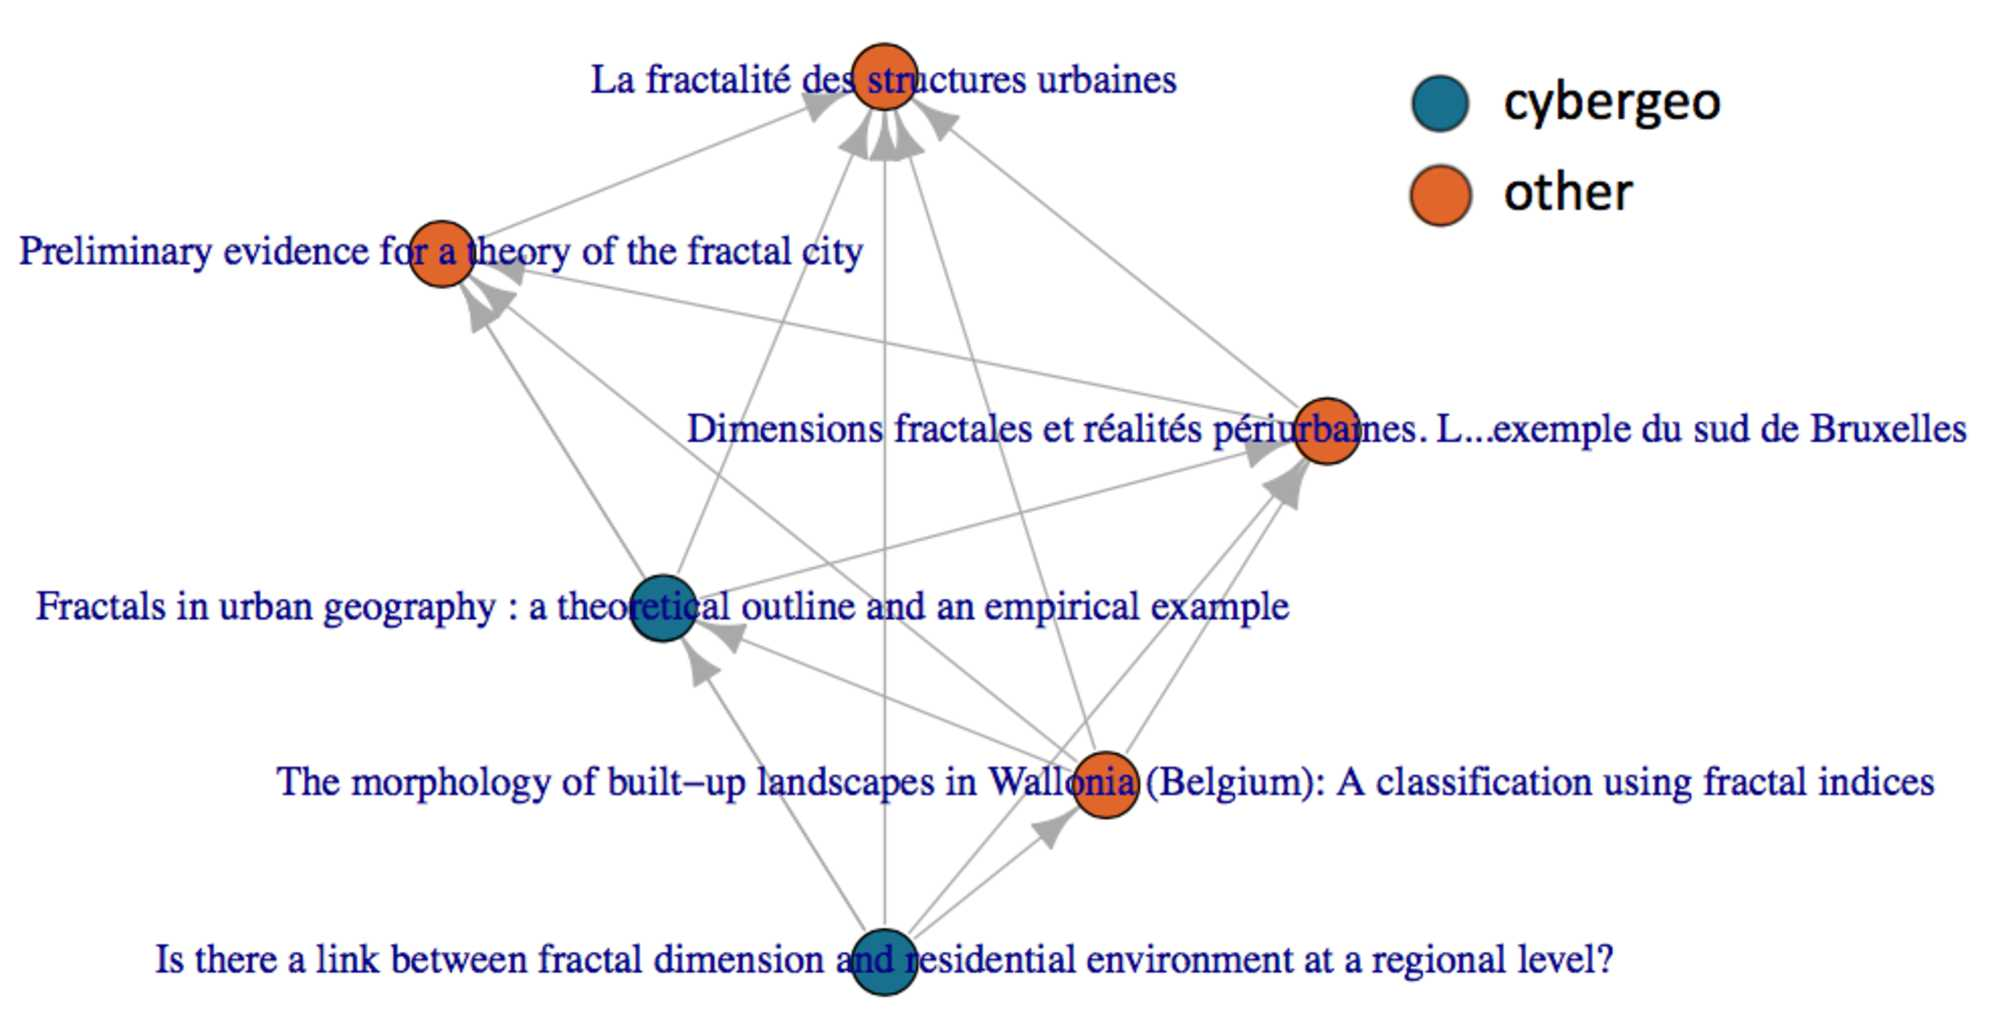
\includegraphics[width=\textwidth]{figures/Fig4.jpg}

}

\sframe{Citation communities}{

% The citation network is a first opportunity to construct endogenous disciplines, by extracting citation communities. More precisely, this step aims at finding recurrent pat- terns in citations that would define a field by its citation practices. In order to be con- sistent with the particular data structure we have (missing incoming citations for sub- corpuses at maximal depth), we filter the network by removing all nodes with degree smaller than one. This ensures that the nodes kept are either at least cited by an other node (and thus there are no missing edges for these nodes) or cite at least two other nodes, what can make “bridges” between sub-communities. The resulting network has a size of |V| = 107,164 nodes and |E| = 309,778 edges. The citation network is visualized in Fig. 5. We use a standard modularity optimization algorithm to identify communities (Blon- del et al. 2008) in the citation network. This Louvain algorithm is applied on the cor- responding undirected network following the elementary solution for community detec- tion in directed networks (Malliaros and Vazirgiannis 2013). It provides 29 communities with a modularity of 0.71, which means that communities are highly integrated [gener- ally, values above 0.4 are already considered as strongly clustered (Newman 2006)]. In comparison, a bootstrap of 100 randomisations of links in the network gives an average modularity of −1.0 × 10−4 ± 4.4 × 10−4. This bootstrap gives statistical significance to the value we obtained, as the observed modularity is larger by more than four order of magnitude than the standard deviation of this null model. We name the communities by inspection of the titles of most cited references in each. This naming process was done under the supervision of the editorial head of the jour- nal. The 14 communities that have a size larger than 2.5% of the network are: Complex Networks, Ecology, Social Geography, Sociology, GIS, Spatial Analysis, Agent-based Modeling and Simulation (ABMS), Socio-ecology, Urban Networks, Urban Simulation, Urban Studies, Economic Geography, Accessibility/Land-use, Time Geography. These categories do not directly correspond to well-defined disciplines, as some correspond more to methods (ABMS), objects of study (Urban Studies), or paradigms (Complex Networks). Some are “specializations” of others: most papers in Urban Studies can also be classified as Critical and Social geography. This way, we construct endogenous disciplines that correspond to scientific practices (what is cited) more than their repre- sentation (the “official” disciplines). The relative positioning of communities in Fig. 5, obtained with a Force-Atlas algorithm, tells a lot about their respective relations: for example, social geography makes a bridge between Urban Studies and Economic Geog- raphy, whereas the connection between Socio-ecology and Urban simulations is done by GIS (what can be expected as geomatics is an interdisciplinary field). GIS also separates and connects two subfield of Ecology, on one side more thematic studies on ecologi- cal habitats, and on the other sides statistical methods. These relations already inform qualitatively patterns of interdisciplinarity, in the sense of integration measures. We will also in the following use these communities to situate the semantic classification.
%Regarding the validity of the map we obtained, the content and structure of our data- set does not allow us to give an exogenous validation using existing techniques Boyack et al. (2005). We rely for the validity of our approach (1) first on the expert knowl- edge used to name the communities; (2) secondly on the high values of the modularity which witness a strong endogenous relevance; (3) the fact that we do not aim to produce exhaustive maps of the discipline, but only to explore the neighborhood of the origin journal; and (4) the low sensitivity to network perturbations as it is developed below in the sensitivity analysis section.


\begin{center}
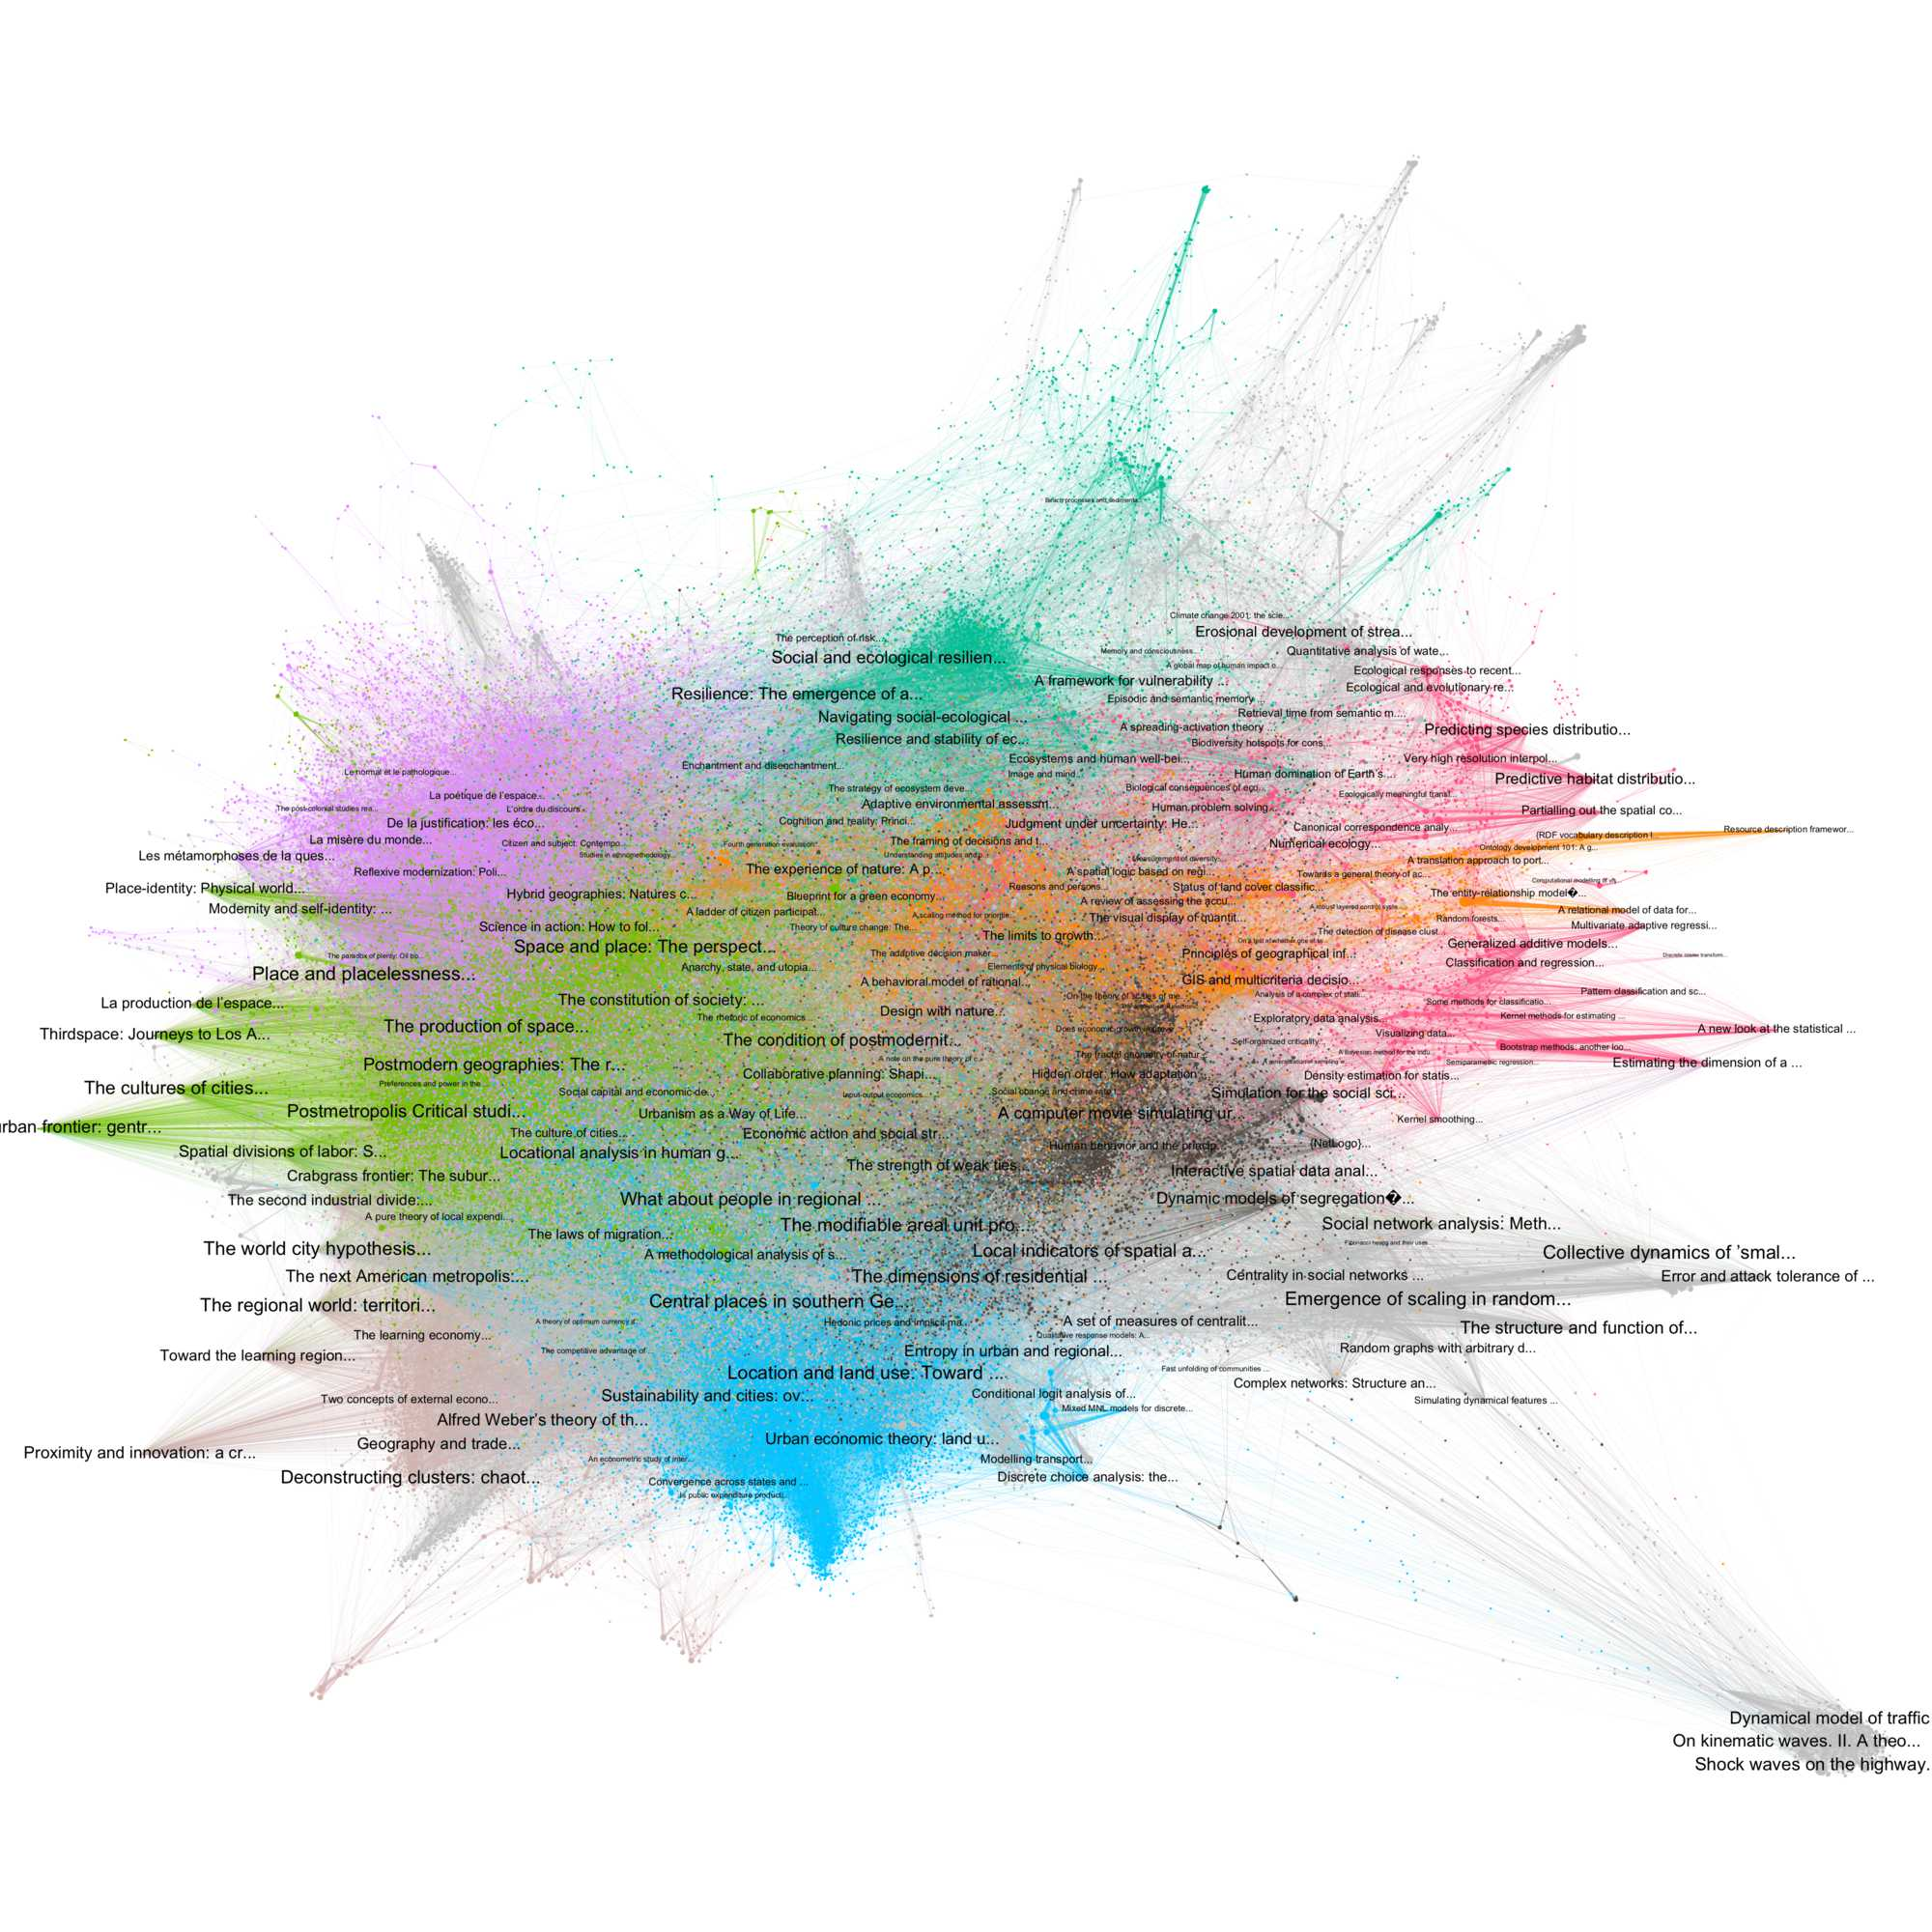
\includegraphics[width=\textwidth,height=0.7\textheight,trim=0 0 0 2cm]{figures/Fig5.jpg}
\end{center}

\footnotesize
\textit{Louvain algorithm community detection to construct endogenous citation communities (modularity of 0.71)}

}


\sframe{Semantic network}{

% We now turn to the methodological details for the construction of the semantic clas- sification. This step adapts the methodology described by Bergeaud et al. (2017), who construct a semantic classification on patent data. We recall that our corpus with available text consists of around 2 × 105 abstracts of pub- lications at a topological distance shorter than 2 from the journal Cybergeo in the cita- tion network. The first important step is to extract relevant keywords from abstracts. Text processing is done with the python library nltk (Bird 2006). We add a particular treat- ment to the method of Bergeaud et al. (2017), as our corpus is multilingual: language detection is done with the technique of stop-words (Baldwin and Lui 2010). We also use a specific tagger (the function allowing the attribution of grammatical function to words), TreeTagger (Schmid 1994), for languages other than English. To summarize, the keyword extraction workflow goes through the following steps:Language detection is done using stop-words, by selecting the language which nltk stop-words dictionary has the most words in common with the current text. 2. Pos-tagging (detection of word functions) and stemming (extraction of the stem) are done differently depending on language: – English: nltk built-in pos-tagger, combined to a PorterStemmer – French or other: use of TreeTagger (Schmid 1994) 3. Selection of potential n-grams (keywords of length n with 1 ≤ n ≤ 4) following the given grammatical rules to identify noun phrases: for English⋂{NN ∪ VBG ∪ JJ}(which cor- respond respectively to noun, gerund verb, adjective), and for French ⋂{NOM ∪ ADJ} (respectively noun, adjective). More elaborated procedures to infer grammatical rules for noun phrases by learning from corpuses do exist (Cardie and Pierce 1998), but are devised to gain knowledge on grammar specifically. We follow the simple procedure of Chavalarias and Cointet (2013) with these simple fixed rules for noun phrases, similarly to Kumar and Srinathan (2008) without the use of heavy additional dictionaries for filtering. Other languages are a negligible proportion of the corpus and are discarded. 4. Estimation of the relevance n-grams, by attributing a score following the deviation of the statistical distribution of co-occurrences to a random distribution. 
% We keep at this stage a fixed number KW of n-grams, based on their relevance score, that will be designated as the relevant keywords. We find that for large values of KW , results are not sensitive to the total number of keywords, and take a reasonably large value for com- putational performance, KW = 50, 000. We construct the co-occurrence matrix of the rel- evant keywords. This co-occurrence matrix provides the semantic network as its adjacency matrix: nodes are keywords, and they are linked according to their co-occurrences.

Construction of the semantic network as a co-occurence network between keywords extracted following \cite{bergeaud2017classifying}:

\medskip

\begin{enumerate}
	\item Language detection using stop-words \cite{baldwin2010language}
	\item Part-Of-Speech tagging (\texttt{nltk} or \texttt{TreeTagger} \cite{schmid1994probabilistic}); stemming
	\item Construction of potential n-grams: nouns and adjectives up to size 4
	\item Estimation of n-gram relevance following the deviation to the expected statistical distribution of co-occurences (chi-squared test)
\end{enumerate}



}

\sframe{Sensitivity analysis of the semantic network}{

% We observe the same phenomenon than in Bergeaud et al. (2017), that is the existence of nodes with large degree and not specific to a particular field: for example model and space are used in most of subfields of Geography. We also adapt the original filtering procedure, as we do not have here an exogenous information to calibrate parameters. We assume the highest degree terms do not carry specific information on particular classes and can be thus filtered given a maximal degree threshold kmax. We keep the second filter on a minimal edge weight threshold 𝜃 . We add the supplementary constraint that keywords are also filtered on a document frequency window fmin,fmax (number of references in which they appear), what is slightly different from network filtering. A sensitivity analysis of resulting network topology to these four parameters is presented in Fig. 6. Given a filtered network, we detect communities using modularity optimization as before for the citation network. Various properties of the network can be optimized, and we look in particular at its size (number of keywords after filtering), the optimal modularity, the number of communities, and the balance between their sizes (defined as a concenration index This multi-objective optimization problem does not have a kk kk unique solution as objectives are contradictory in a complex way, and a compromise point must be chosen. Indeed, one can obtain a very high modularity but with a small network which will finally cover only a small fraction of the corpus, whereas a large network yields lower modularity values as shown in Fig. 6. The process is similar for other indicators. We take a compromise point between modularity and network size, with a high balance and a reasonable number of communities, given by kmax=1200,𝜃w=100,fmin=50,fmax=10000. This point was taken on the com- promise line between modularity and network size (roughly around the line link- ing (𝜃w = 50, kmax = 400) with (𝜃w = 100, kmax = 1200)), with a high balance (taking kmax ≥ 1000) and not too much communities. These values give a network of size 2868, with 18 communities and a modularity of 0.57. Note that the small proportion of keywords in French is always separated from the rest of the network as they cannot co-occur with English keywords, and that with these param- eter settings no French keywords are kept. All communities described in the following therefore contain only keywords in English.

\justify

\vspace{-0.5cm}
Additional filtering procedure to remove relevant but common keywords: filter on edge weight and maximal degree; values chosen based on multiples objectives including modularity and network size.

\medskip

\centering

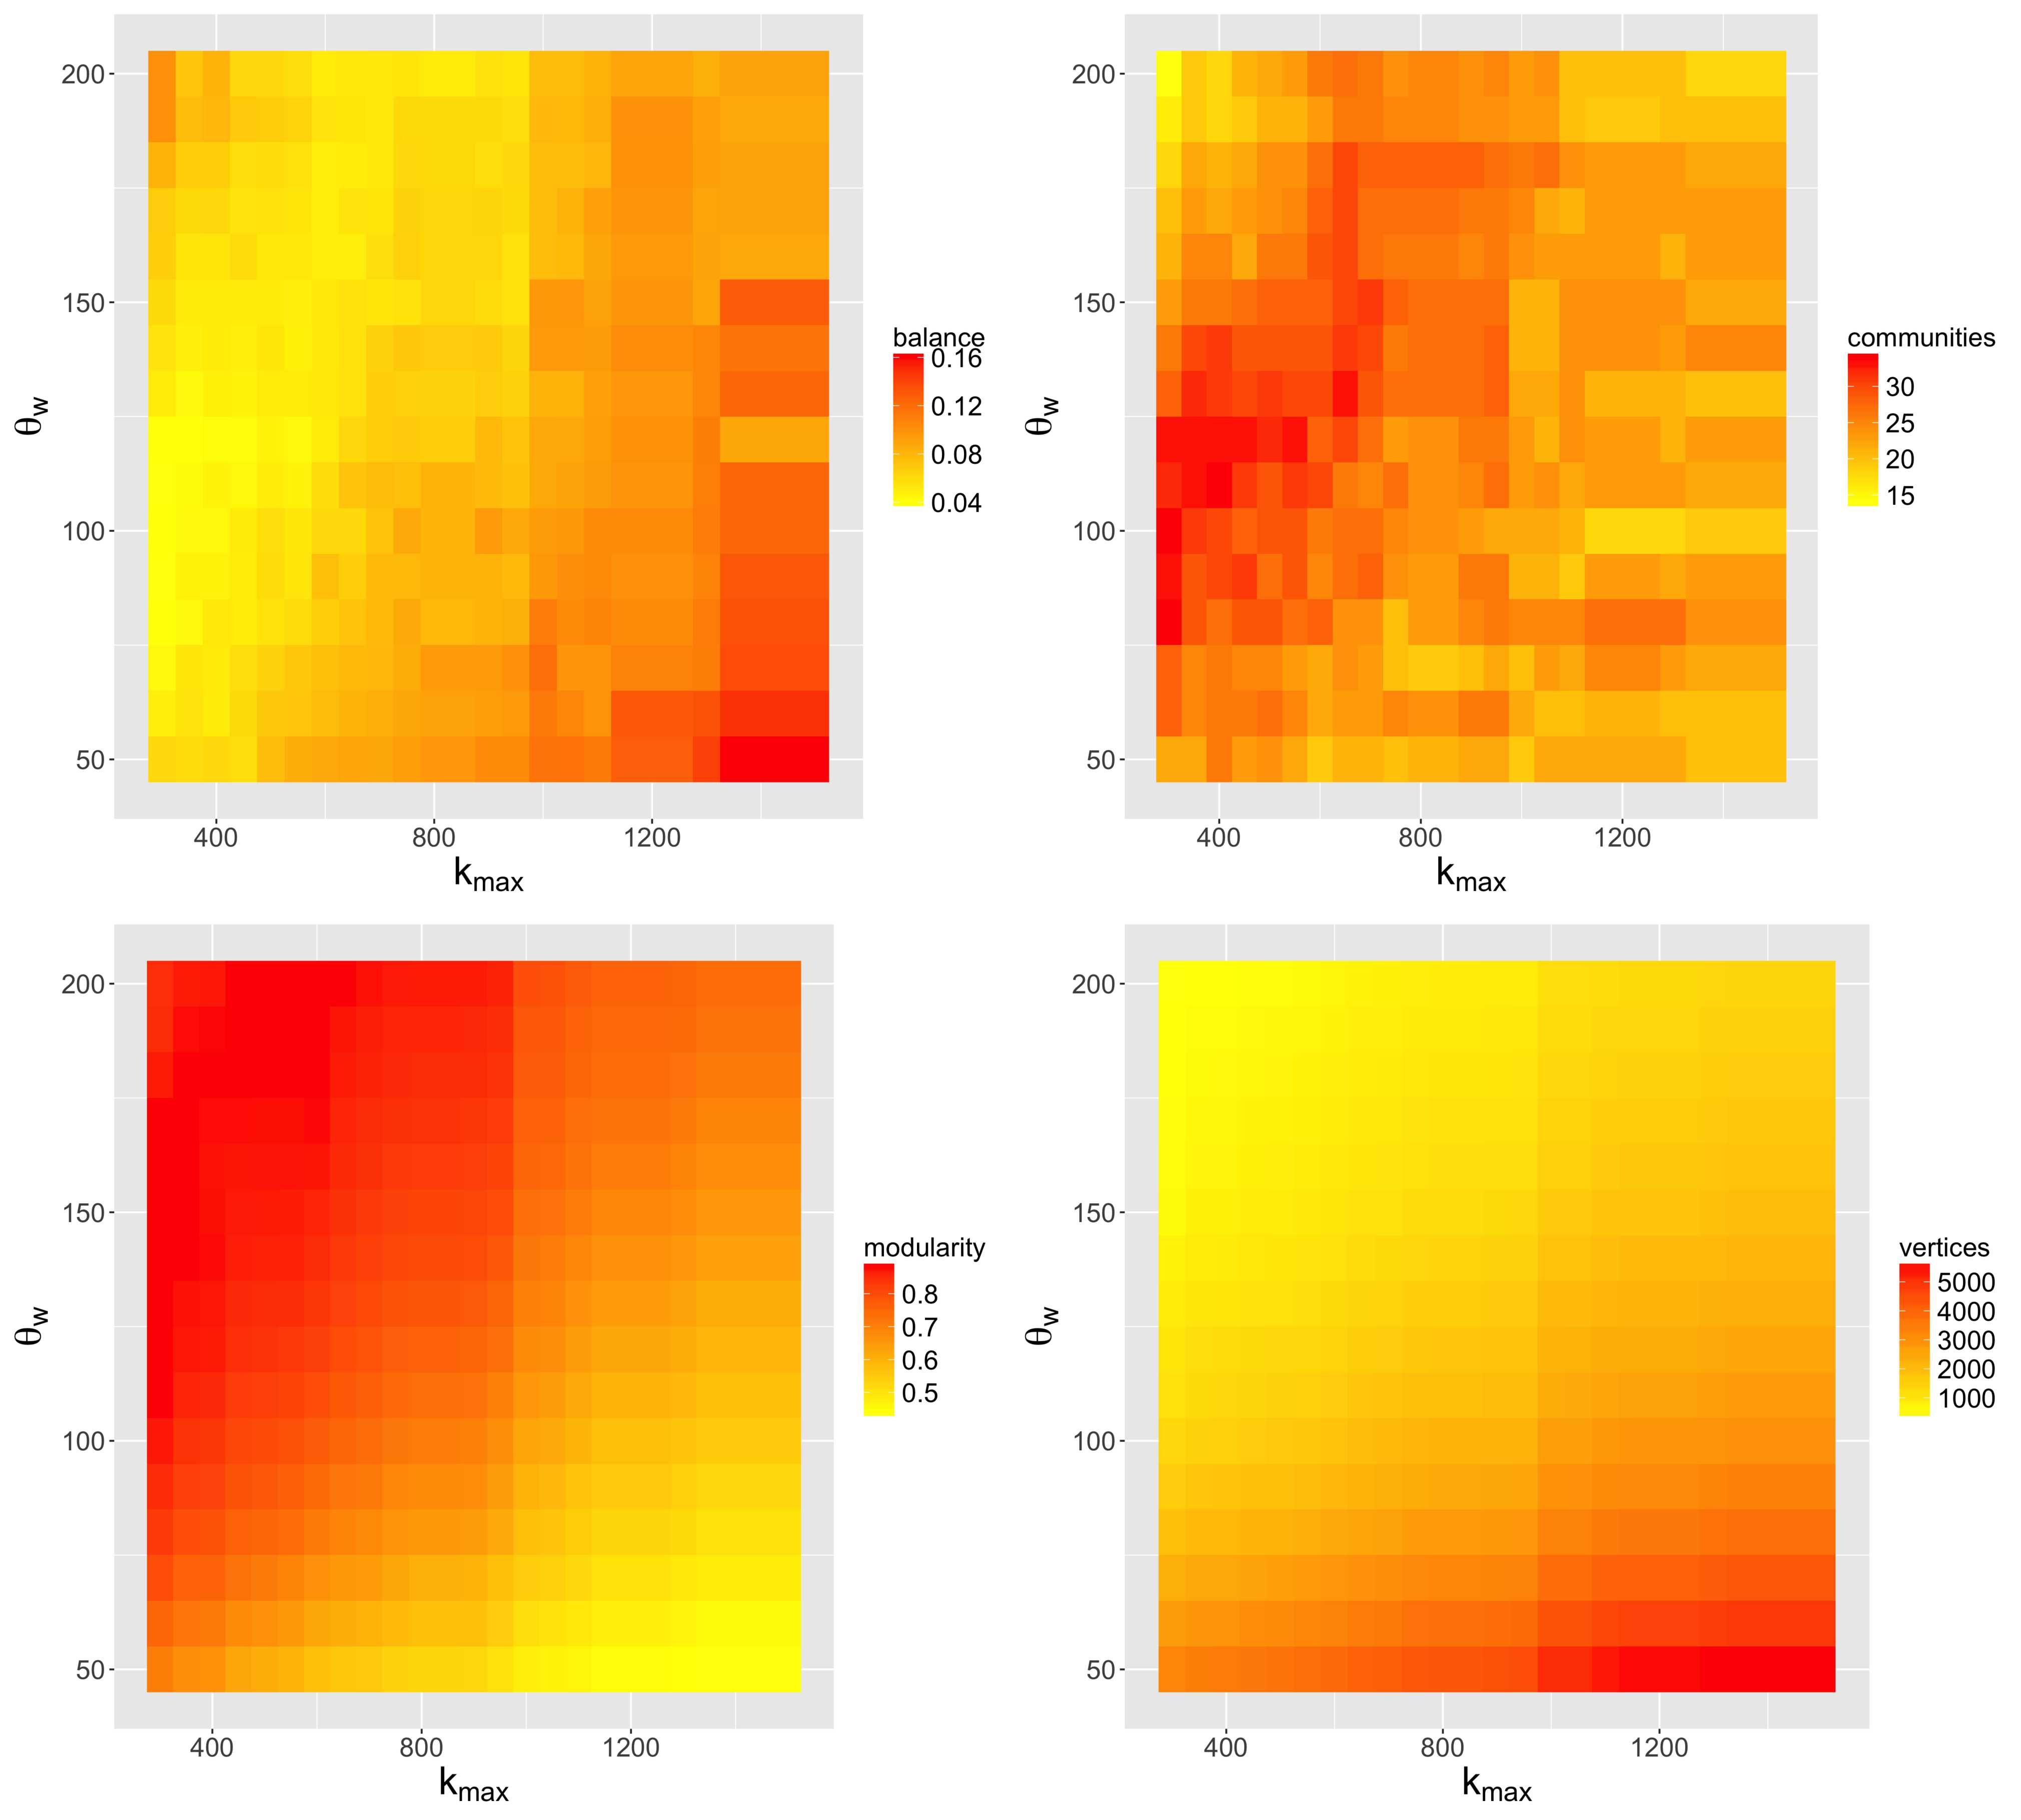
\includegraphics[width=0.6\textwidth]{figures/Fig6.jpg}

}

\sframe{Semantic network visualization}{

\centering

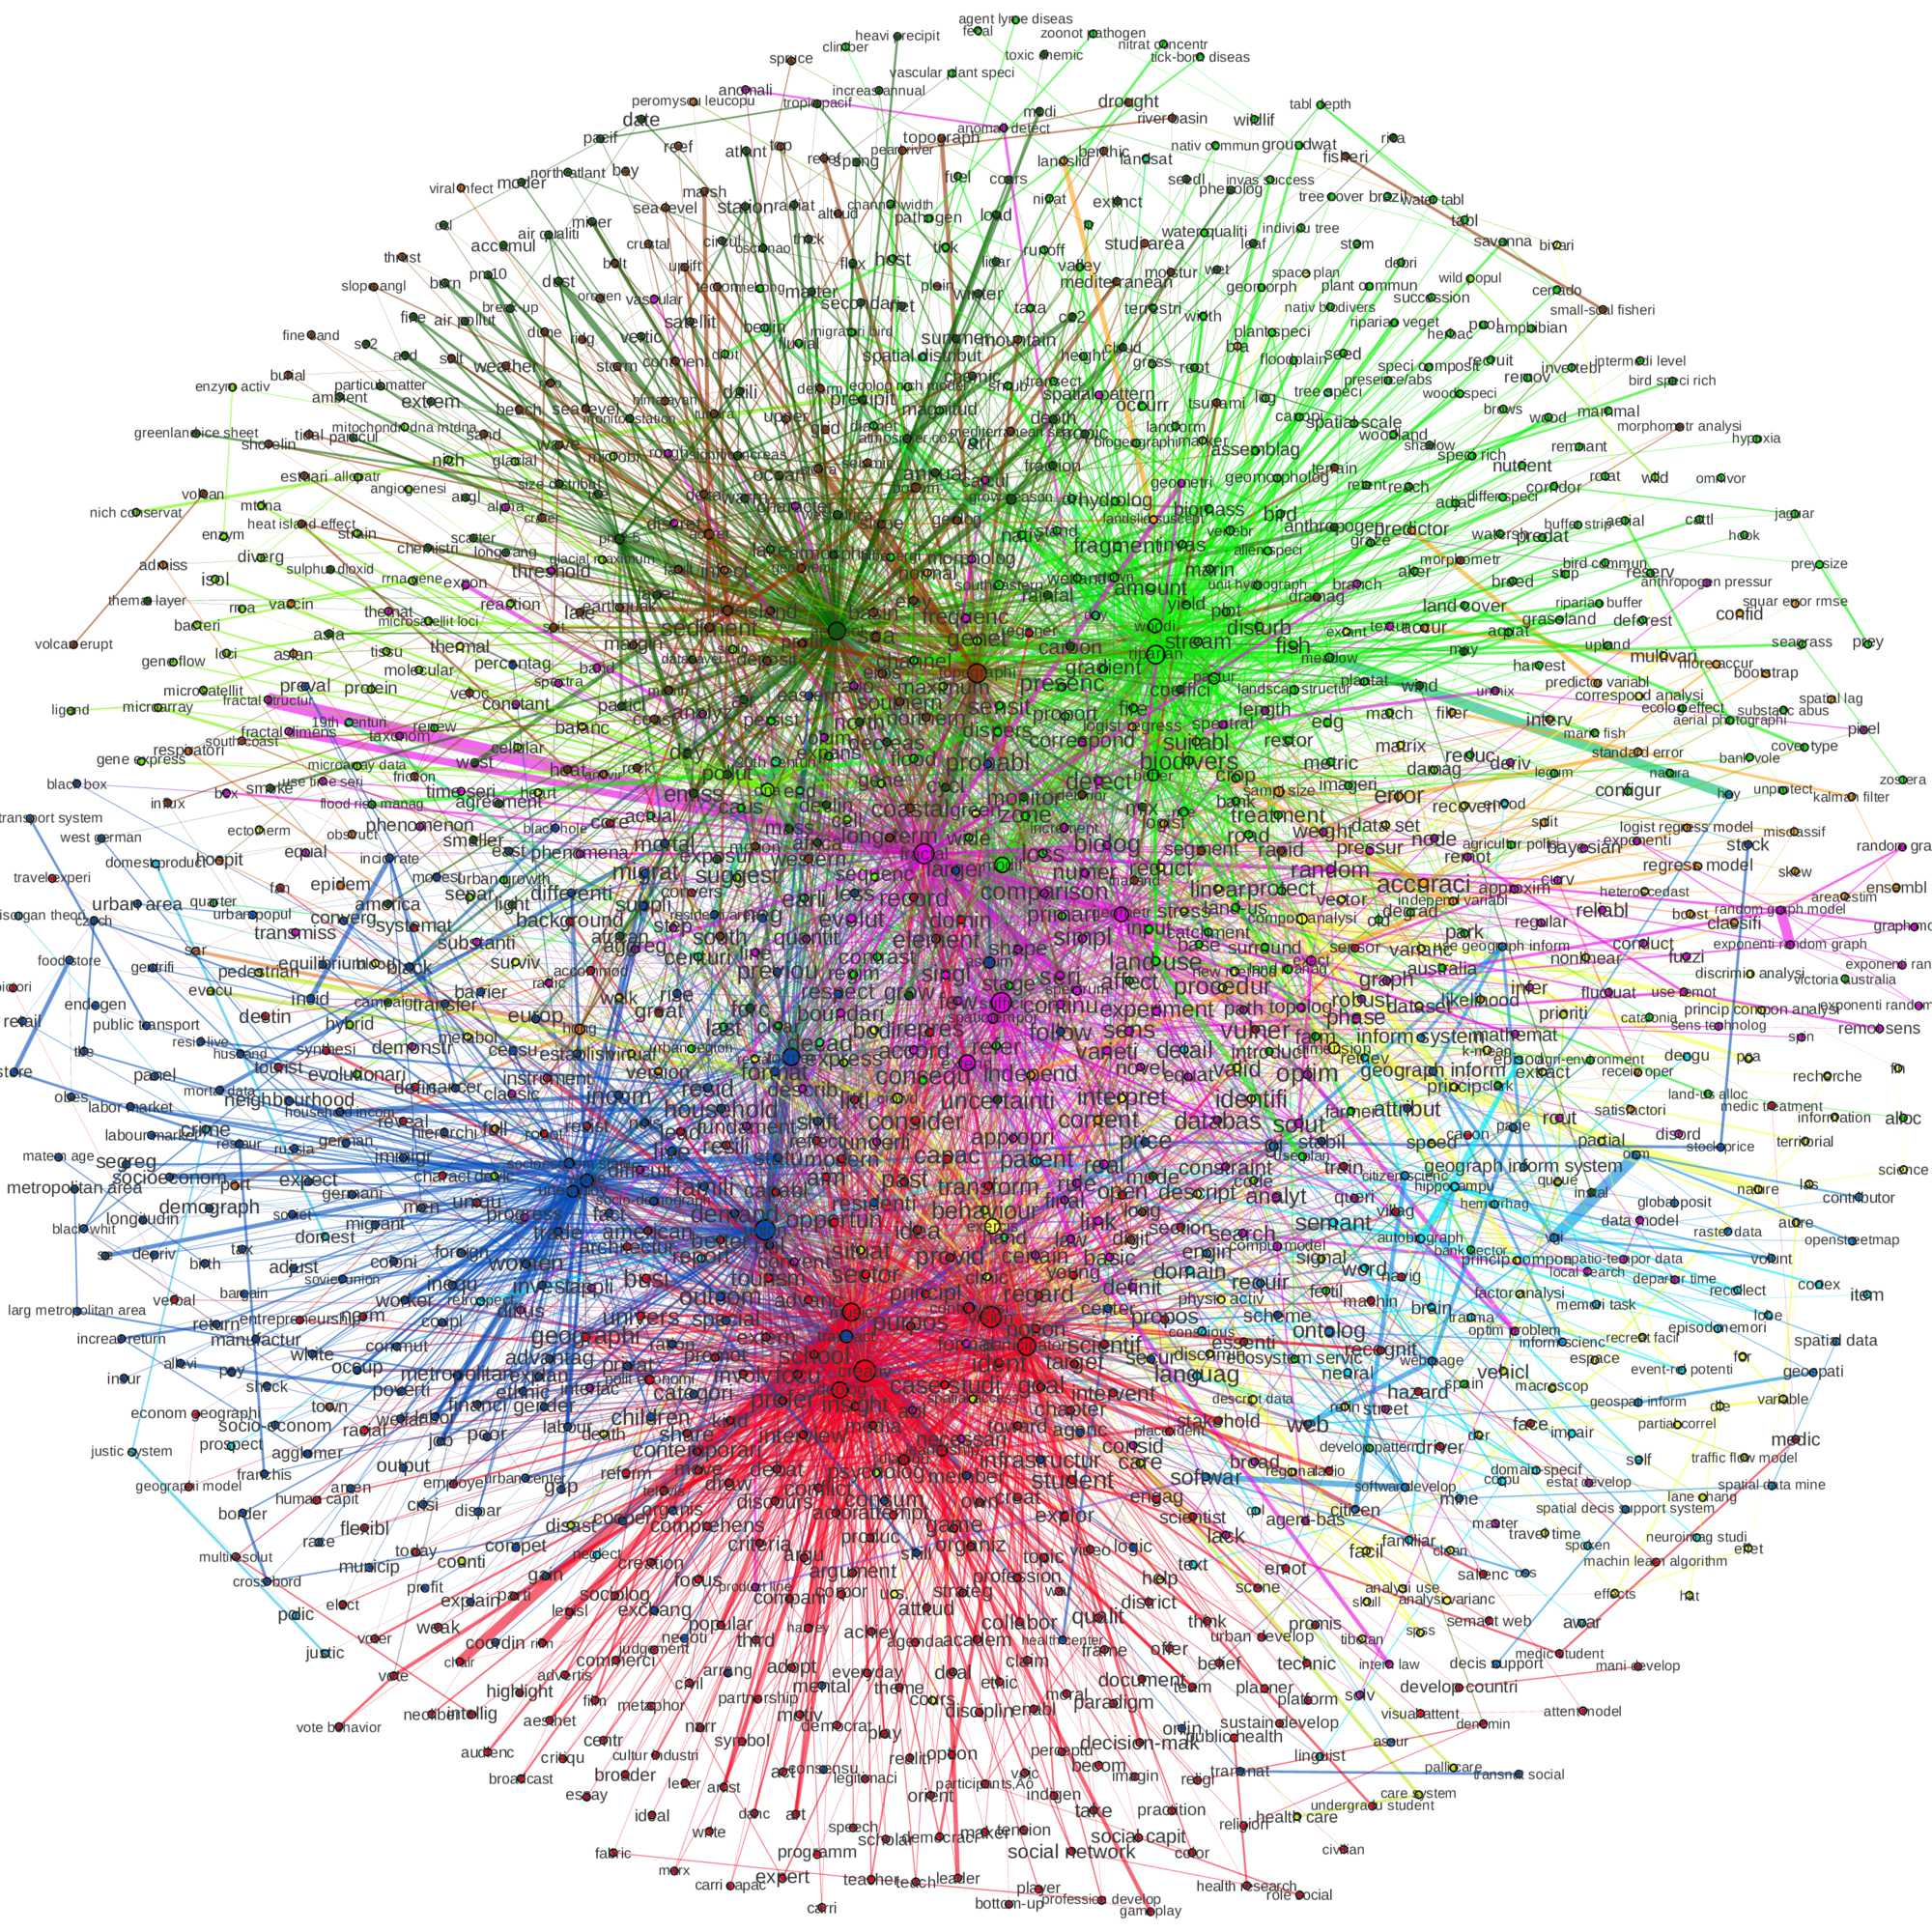
\includegraphics[height=0.9\textheight]{figures/Fig7.jpg}

}



\sframe{Semantic communities}{

% We obtain therein communities in the semantic network with the optimized filtering param- eters. At the exception of a small proportion apparently resulting from noise (representing less than 10 keywords in 3 communities that we remove, i.e. 0.33% of keywords), commu- nities correspond to well-defined scientific fields, domains, or approaches. Naming is also done by inspection of the most relevant keywords in each community, in order to stick here to a certain level of supervision. Table 1 summarizes the communities, giving their names, sizes, and corresponding key- words. The most important community is related to issues in political science and critical geography, what could have been expected as several previously obtained citations commu- nities (Social geography, Urban studies) deal with these issues. We then obtain a large clus- ter of terms related to biogeography, that must correspond to publications in Ecology and Socio-ecology identified before, together with a community in Environment and Climate. In a way similar to the citation communities, but more pronounced here, we obtain endogenous “disciplines” that can correspond to real disciplines, to methodologies, to object of studies. This classification thus also unveil effective scientific practices, here in terms of semantic content. A class here related to complex systems can be associated to a paradigm and various approaches that were separated in the citation communities: agent- based models and complex networks for example. On the contrary, some studies that were gathered in a large domain before can be precisely differentiated in the semantic network, such as microbiology and health here that are used by studies related to socio-ecology or ecology in the citation network. Some very specific domains appear here as they have very few connections in their actual semantic content: for example, Geography of crime is very precise and disconnected from other communities. We show in Fig. 7 a visualisation of the semantic network, in which the positioning of communities, induced by a Fruchterman–Reingold algorithm [that we use here to have a more precise layout in the relative positioning compared to Force Atlas (Jacomy et al. 2014)]. The bridging between distant disciplines is done quite differently compared to the citation network, and reveals thus qualitatively an other dimension of interdisciplinarity, i.e. the semantics shared by disciplines. Here, the communities corresponding to Economic Geography (blue) and to Critical Geography (red) are close as in the citation network, but are linked to ecology and geomorphology (green and brown) by Complex Systems (magenta), although these were not present as a community in the citation network. Com- plexity methodologies such as Fractals, Scaling (West 2017) or Networks (Newman 2003) are indeed widely used both in social sciences and in physics or biology. The semantic analysis reveals thus that very distant disciplines, that are distant in their citation patterns, are finally close in terms of actual content. This conclusion can naturally subject to the bias that similar terms can correspond to very different ontologies in each disciplines. This actual meaning is partly captured in the embedding of the term in the semantic network, and how it relates to other terms in the semantic network. To what extent ontological prox- imities can be associated to semantic proximities or reconstructed from the network struc- ture is an open question out of the scope of this work. Terms must thus not be dissociated from their context, which in our case is given by the citation network, thus the interest of the analysis below on the relation between classifications.

\centering

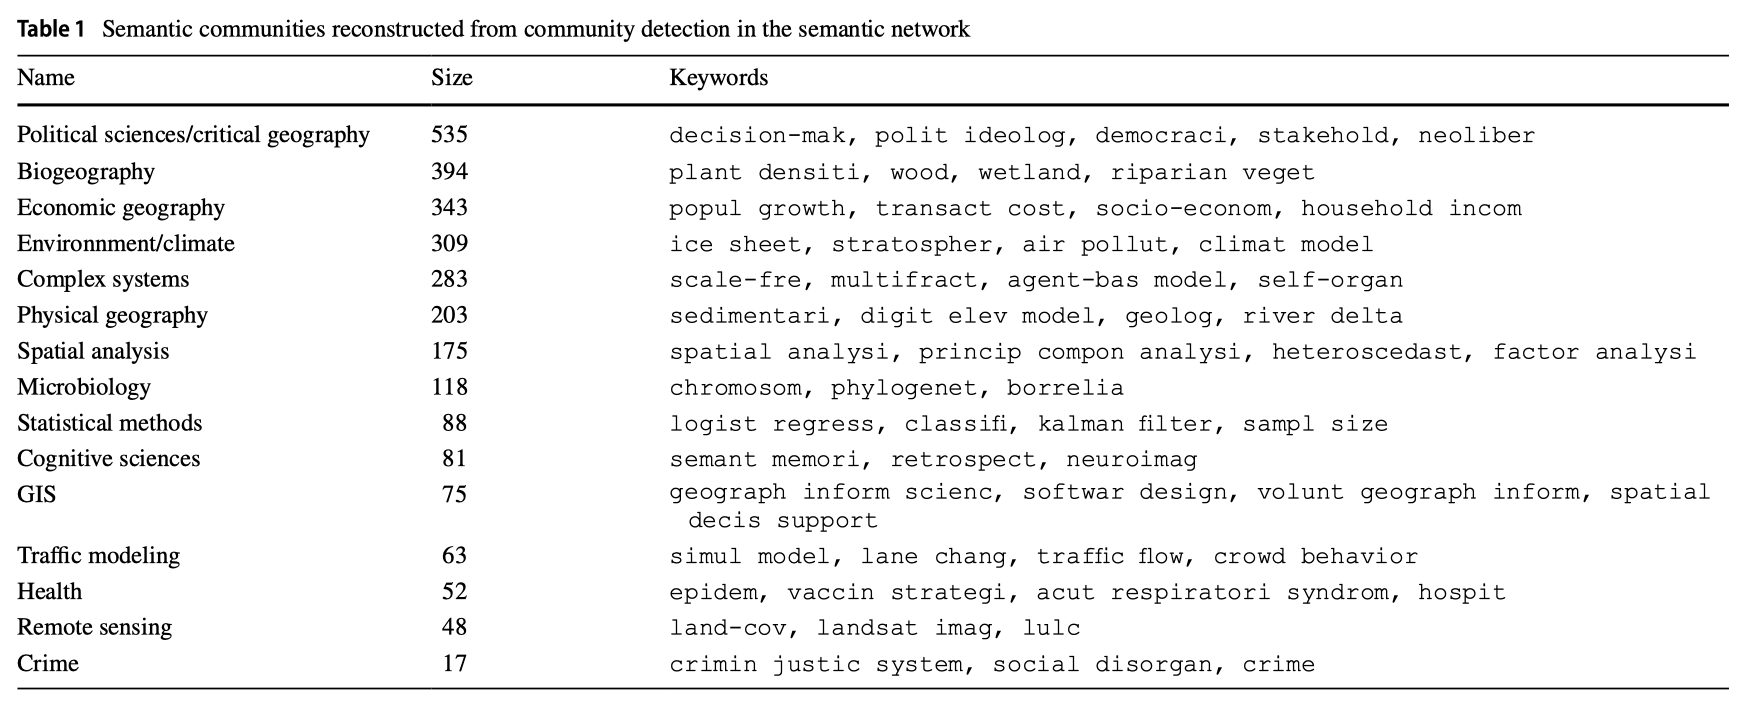
\includegraphics[width=\linewidth]{figures/Tab1.png}

}



\sframe{Interactions between communities}{

% In terms of overlaps between communities, in the sense of co-occurrences of cor- responding keywords within texts of references, we show a synthesis of links between semantic communities in Fig. 8. We see that communities such as Critical Geography and Biogeography are not totally disconnected and share still a certain number of co-occur- rences. More isolated communities can be spotted such as Health and Crime Geographies. Surprisingly, Statistical Methods does not share strong links with other communities, what could mean that articles dealing with methodological issues in this field are rather discon- nected from the field of application, or at least do not describe it extensively. On the con- trary, methods in Complex Systems are organically integrated with the thematic issues they tackle.


\centering

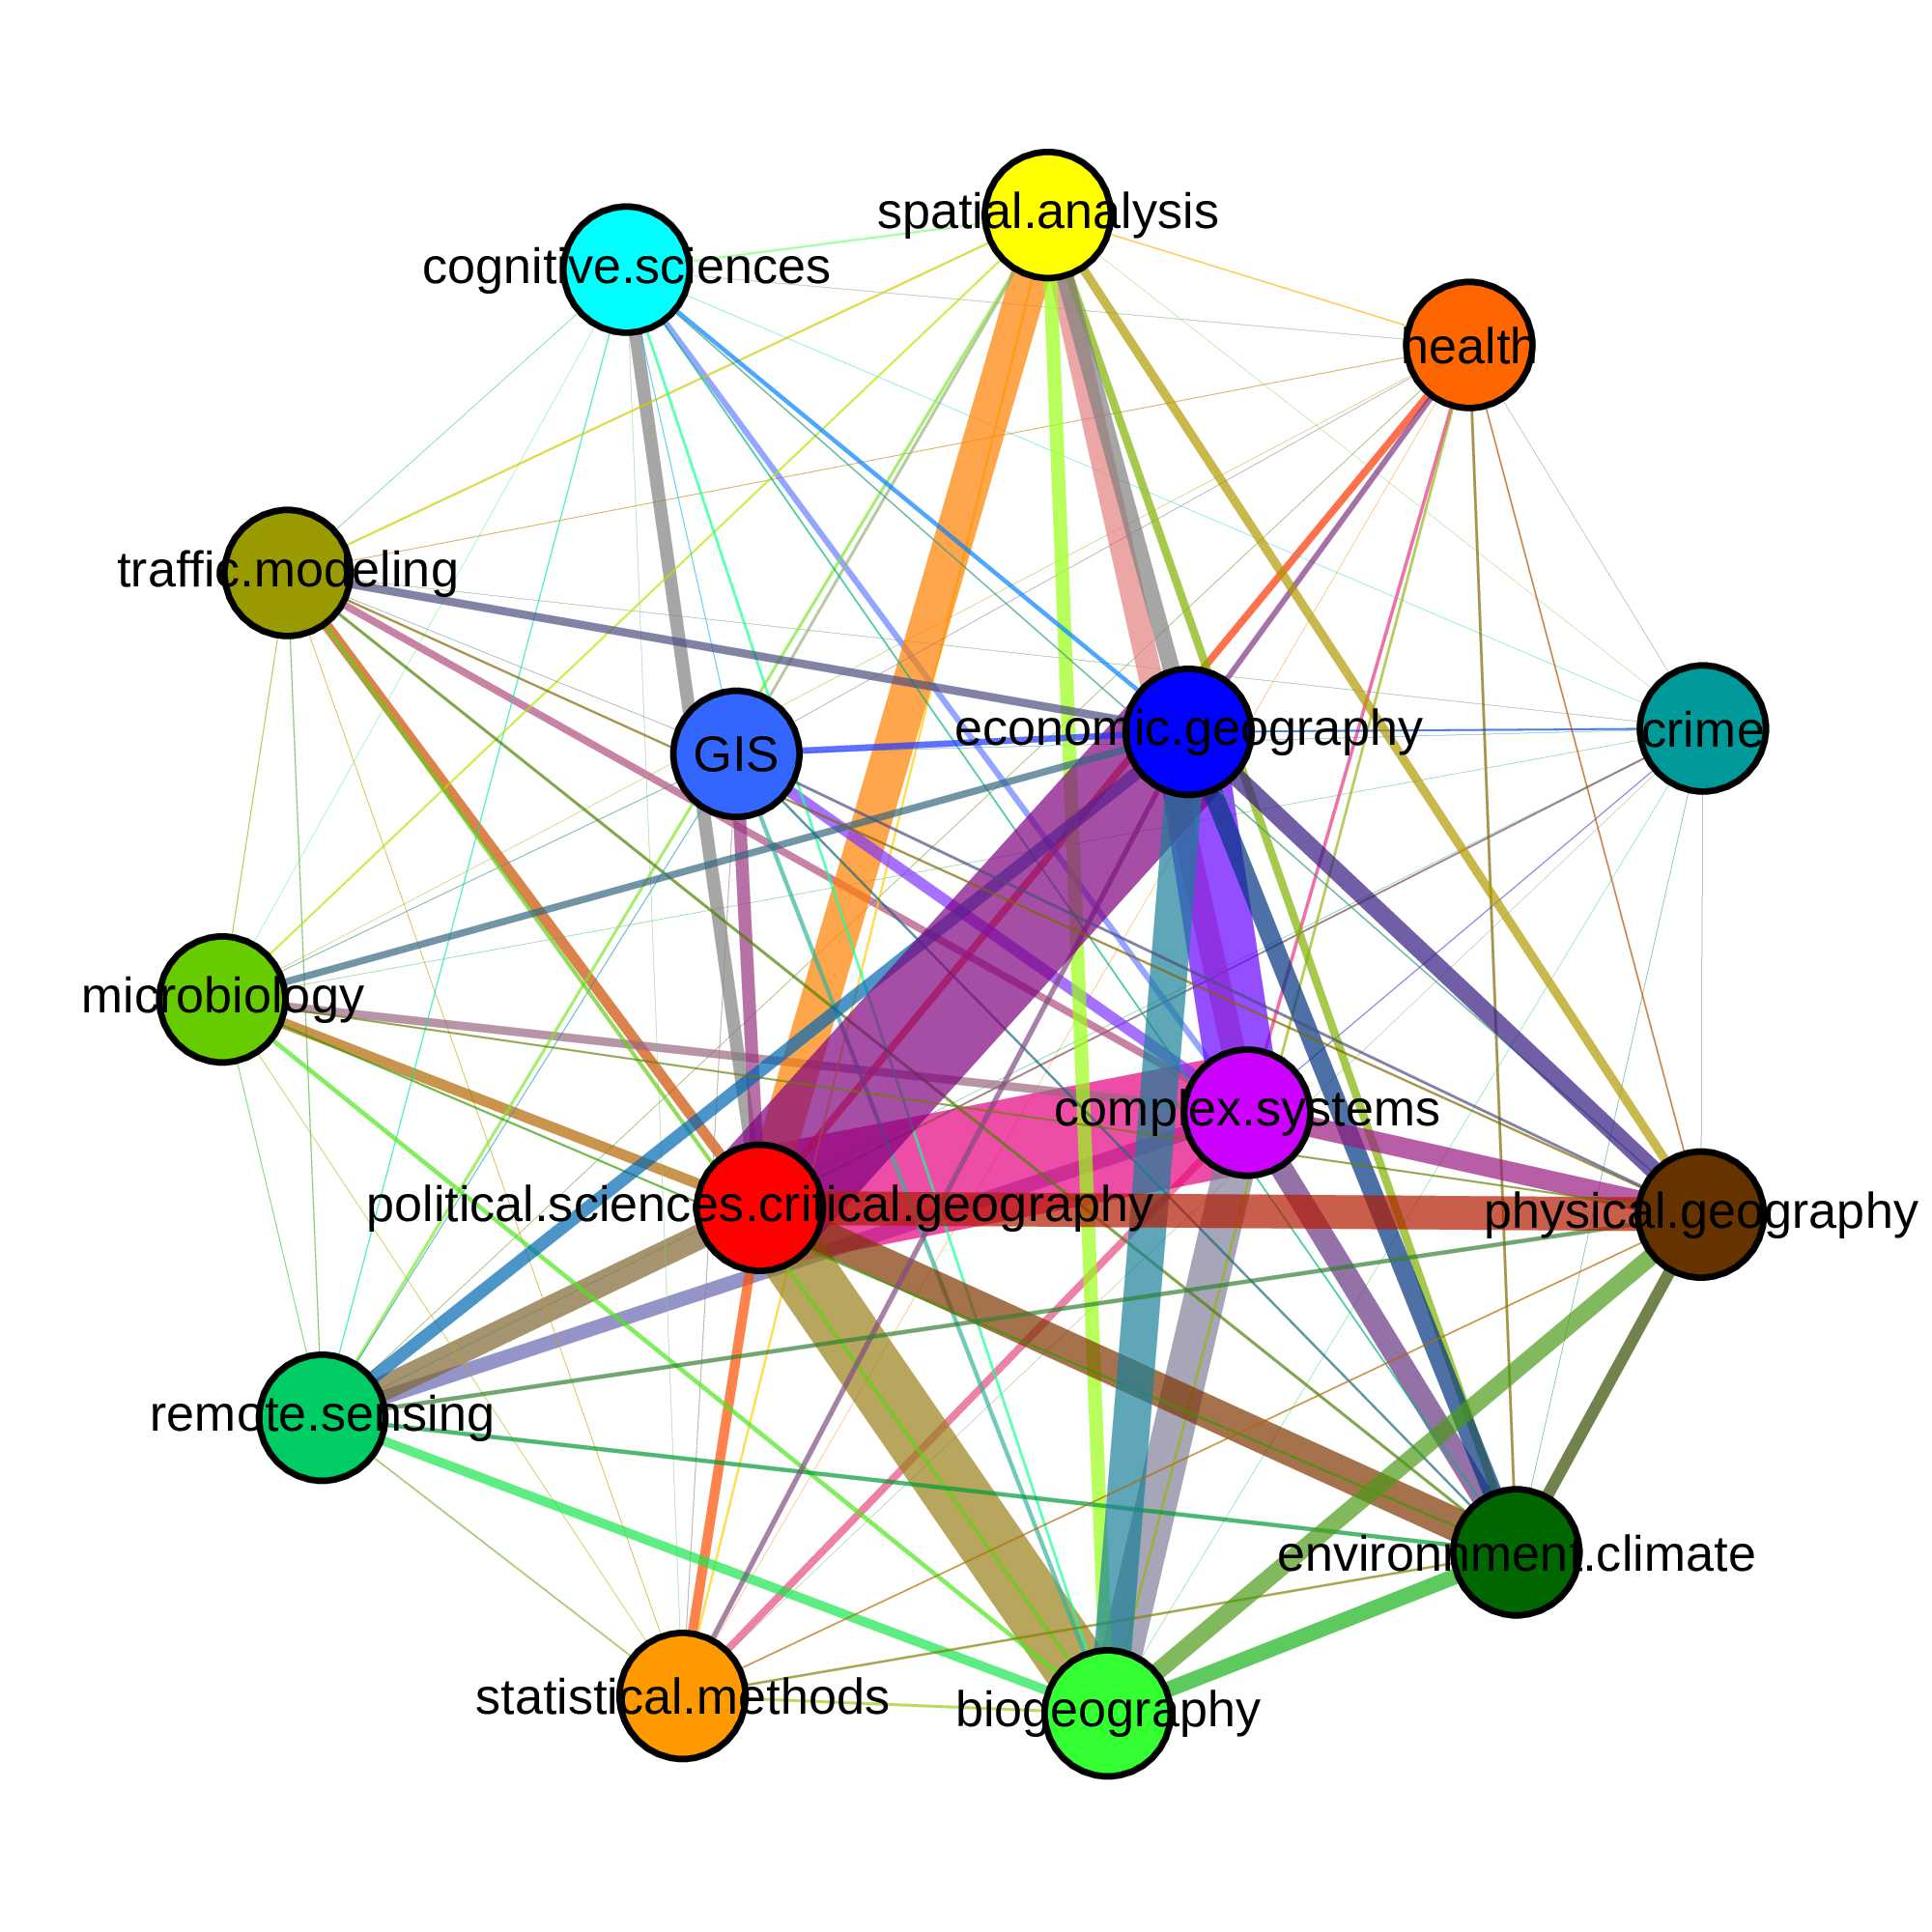
\includegraphics[height=0.9\textheight]{figures/Fig8.jpg}

}


\sframe{Sensitivity to corpus definition}{

% To give a stronger confidence in the results we obtain, we need to study the influence of corpus choice, since (1) our case study is a narrow part of the related disciplines; and (2) the interaction between missing data and the methodology introduced may play a role in the result obtained, that then could be solely due to spurious effects between both. How- ever, our data collection process and classification method were conceived to be used together: using both layers increase the information that can be extracted, since the col- lected data has less information than classical datasets. Our positioning regarding data, i.e. working only with the open dataset in a case of a low data availability, does not allow us to proceed to “ground truth” validations with an exogenous classification. We can however study endogenously the sensitivity of the com- munity structure to the corpus definition, by studying the sensitivity to data removal. This controls the process used by data quality and contributes to the validation of the method, rather independently to the dataset used. The procedure is the following, according to classical approaches to the study of net- work robustness (Trajanovski et al. 2013): working on the citation network, we test the sensitivity of the community structure to entity removal. A fixed proportion r of nodes or edges are removed randomly, and modularity is estimated in the resulting network. This procedure is bootstrapped Nb = 1000 times for each value. Results are shown in Fig. 9, for 0.05 ≤ r ≤ 0.5. We obtain similar qualitative patterns for node and edge removal regarding the form of distributions, but the median modularity slightly decreases for nodes whereas it oscillates for edges. Extreme values are higher for nodes, up to 0.02 difference in absolute value. This remains a very low absolute value, and we find that the community structure has a low sensitivity to data removal, in terms of missing reference (node) or citation link (edge), when going up to 50% of missing data. This gives confidence in the fact that our method is stable relatively independently of the choice of the origin corpus. We also tested the influence of the time window used, since our origin corpus spans between 1996 and 2016. We filter the citation network on fiver-year sliding win- dows covering this span. The size of corresponding subnetworks is relatively stable (|V| ∈ [27866;60474] and |E| ∈ [18839;33892]) and the modularities are higher than the full network (between 0.84 and 0.88) and stable. This suggests that the community struc- ture is stable in time.


\begin{center}
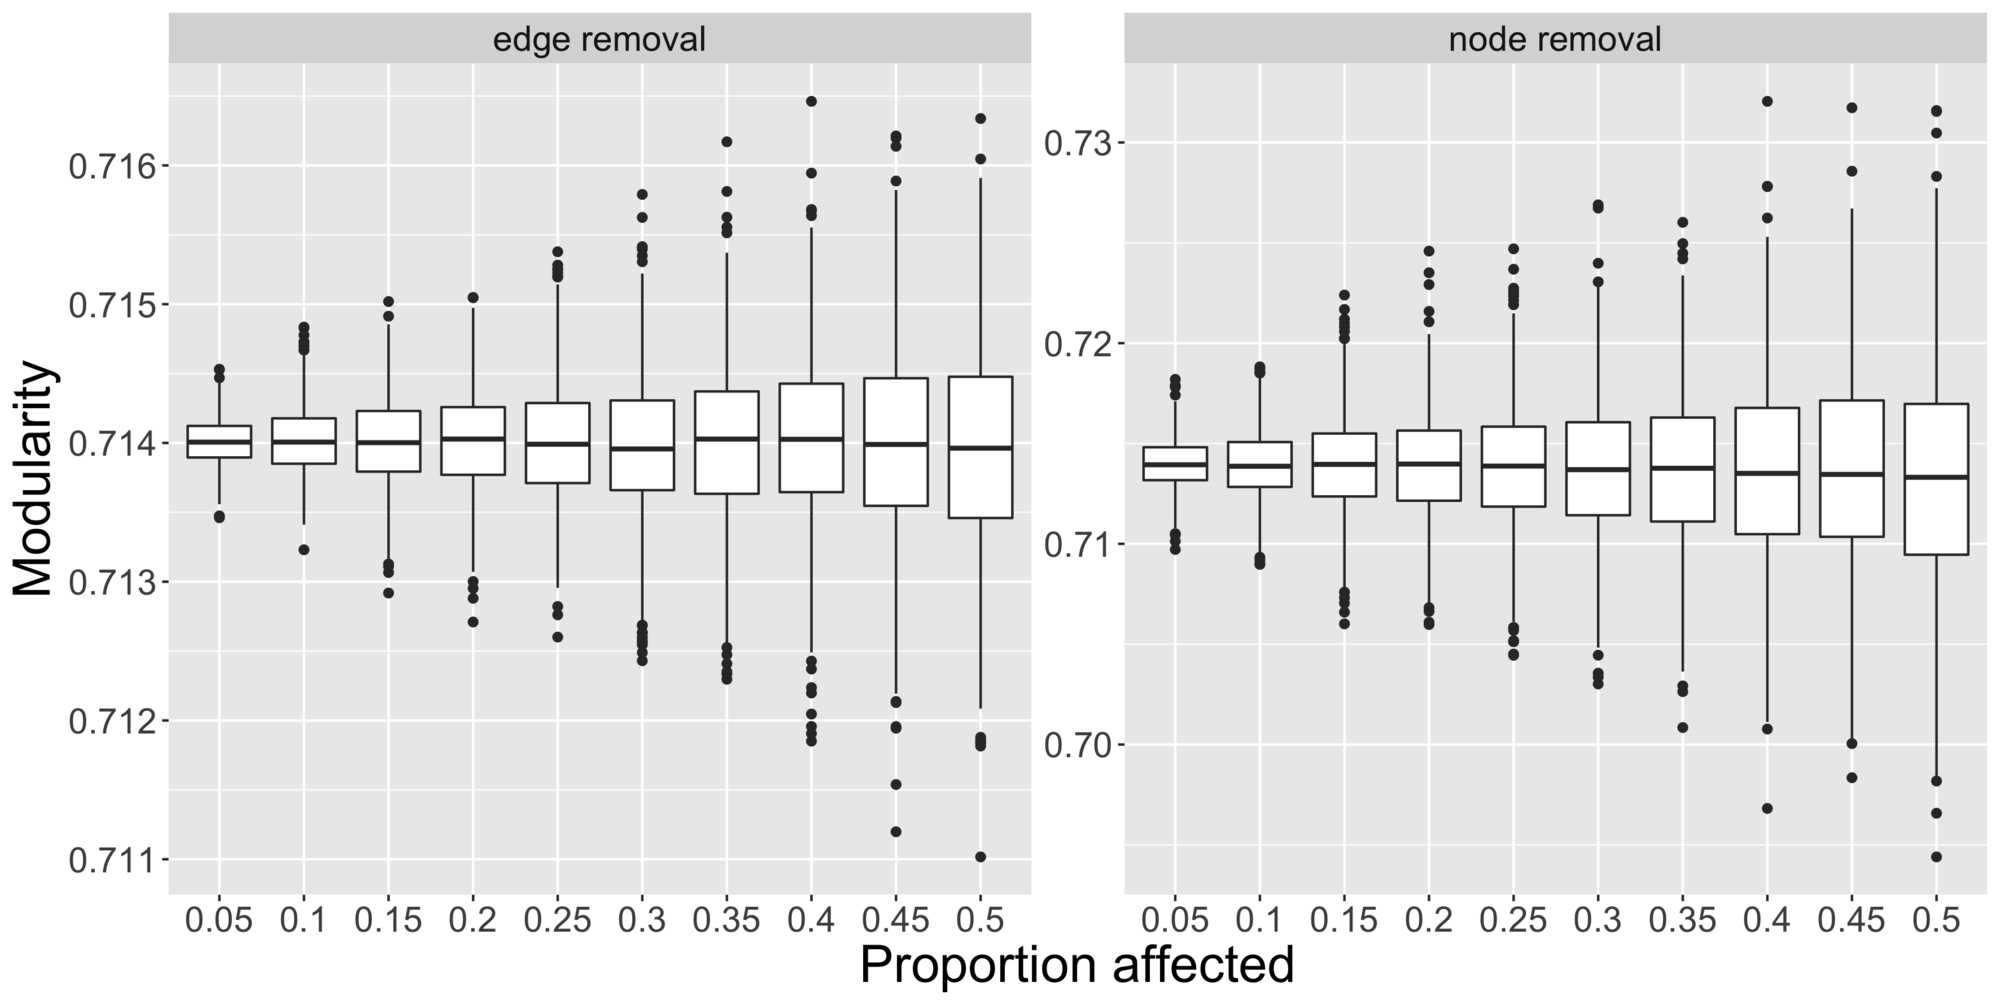
\includegraphics[width=\textwidth]{figures/Fig9.jpg}
\end{center}

\medskip

\textit{Impact of node and edge removal on the optimal modularity of the citation network}


}


\sframe{Semantic composition of citation communities}{

% We can now turn to the study of the relation between classifications. First, a simple way to link them is to look at the semantic content of citation communities. Each reference has a given proportion of keywords within each semantic class, and an average composition in terms of semantic classes for each citation class can thus be computed. We show these composition in Fig. 10. Some expected results are obtained, such as Complex Networks (citation) having the largest part in Complex Systems (semantic), or GIS (citation) the larg- est in GIS (semantic), and similarly for Economic Geography. But the study of patterns that could have not been expected is very informative, and unveils practices of interdisciplinarity. For example, Time Geography (citation) uses as much GIS (semantic) as GIS (citation), what means that they should be using the corre- sponding methods and tools to study the thematic question of spatio-temporal trajecto- ries of geographical agents. The most important in terms of political science (semantic) are Urban Studies, what suggest a convergence of the City as an object of study and of the disciplines of Political Science and Critical Geography. Also interestingly, the cita- tion communities using most biogeography are Ecology (what could have been expected) and ABMS, confirming again the role of the thematic application in complex systems methodologies.

\centering

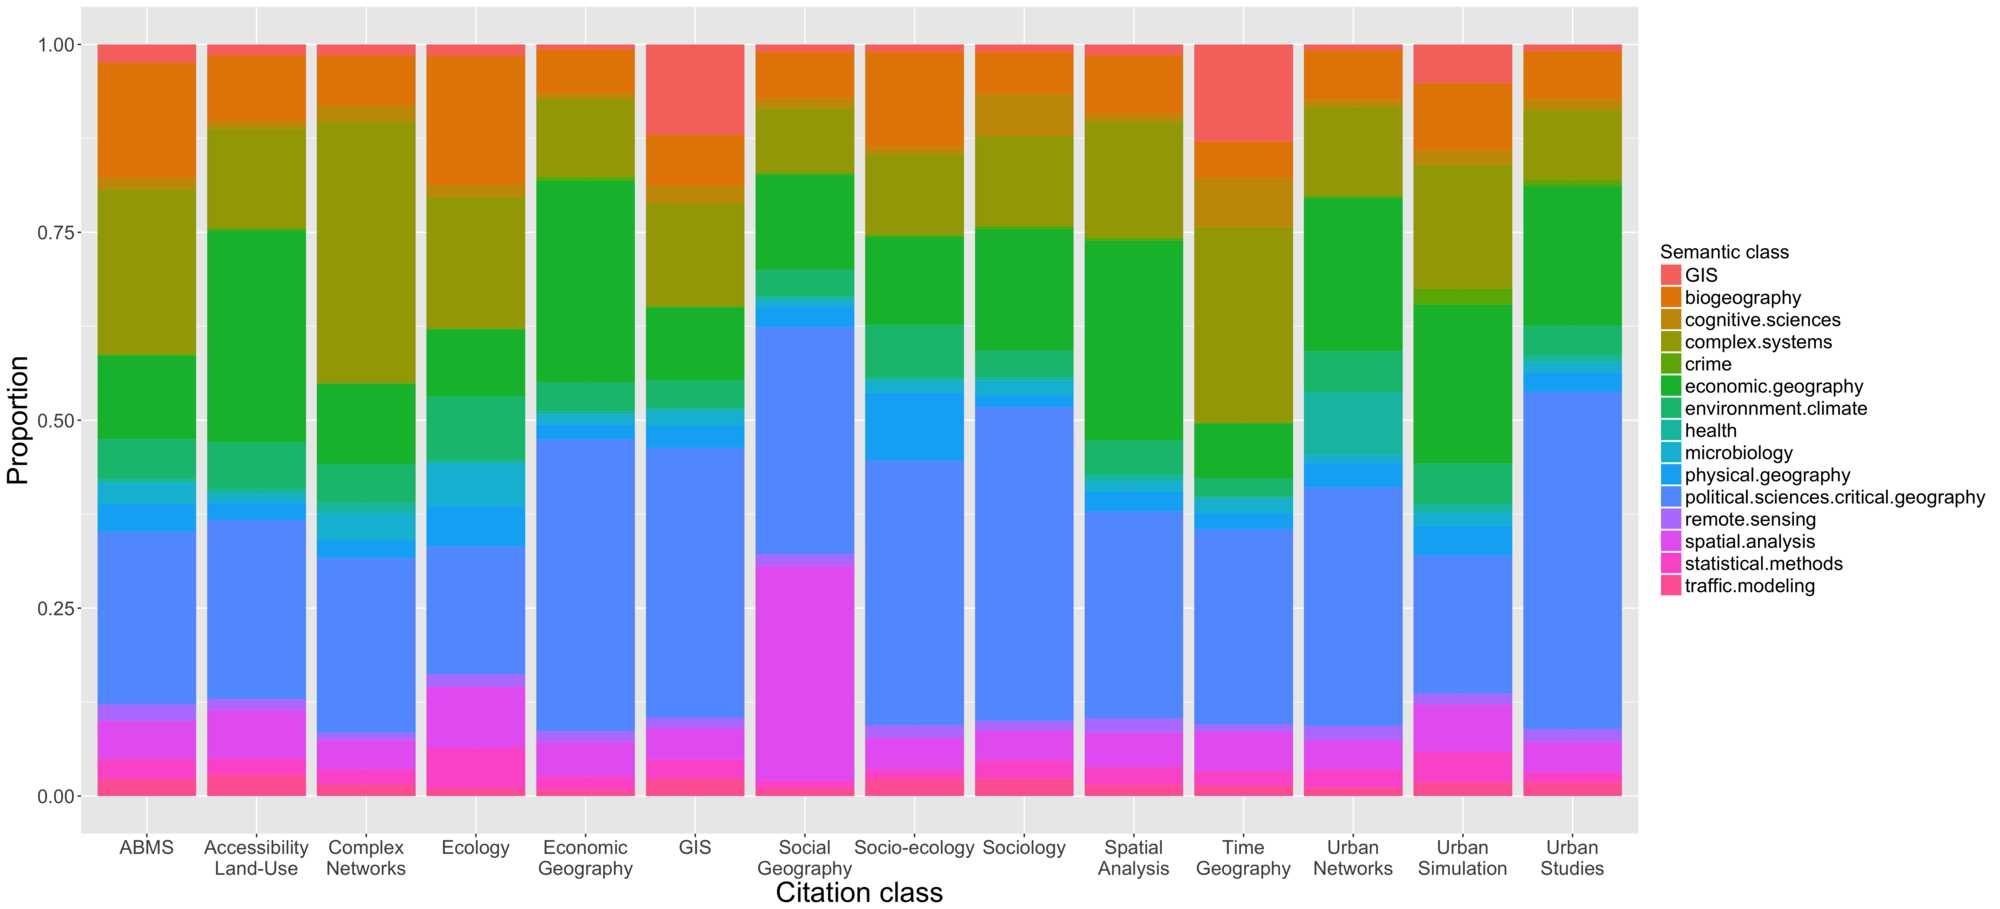
\includegraphics[width=\textwidth]{figures/Fig10.jpg}


}


\sframe{Measuring interdisciplinarity}{


% We had up to now a qualitative view on interdisciplinarity patterns, by looking at the rela- tive localisation of communities within the citation and semantic classifications, and the relation between the classifications. We propose now to look at quantitative measures of interdisciplinarity, for each classification. More precisely, for a given classification C ∈ {Citation, Semantic} a reference i can be viewed as a probability vector (p(C)) on classes j that give for each class the probability to belong to it. Given this setting, we measure interdisciplinarity of one reference using Her- findhal concentration index (Porter and Rafols 2009), that can also be called an originality index. We define originality as (C) ∑ (C)2 oi =1− pij (1) j For the semantic classification, probabilities are defined as the proportion of keywords of the abstract within each semantic class. With the deterministic citation classification, each reference has only one class and the originality index is always 0. Therefore in order to be able to compare the two classification, we associate a probability to each citation class for each article as the proportion of citations received from this class. The index introduced is original, and measures interdisciplinarity as how a reference is used by different disciplines in its lifetime. Indeed, Eq. 1 yields higher values for more evenly distributed probabilities. When used with semantic probabilities, it translates the originality in terms of language used, whereas with the citation probabilities, it gives the originality in terms of domains using the reference.We show in Fig. 11 the statistical distribution for both indexes o(Semantic) and o(Citation), stratified by citation class. This allow a direct comparison between the two and also an indirect comparison by the variation of semantic distribution between citation classes. For the distribution of semantic originalities, all citation classes exhibit a similar pat- tern, that is a peak around large values and a smaller peak at zero. It means that either references are highly specialized and have keywords in one class only, or they use keywords from different classes in a quite even manner (for comparison, an abstract with half keywords in a class and half in an other gives an originality of 0.5). The most original, i.e. the most mixed, citation class, is Complex Networks, with a distribution clearly detached from others, what would confirm their use as a method with a lot of dif- ferent problems. Social Geography is from far the less original, with a large number of single class references, and an average far lower than other classes, what would mean an increased presence of compartmentalization within the associated disciplines. In terms of citation originality index, the global picture is fundamentally different, as average originality indexes are all lower than 0.4 and most of distributions show their mode in 0, meaning that most references are only cited by their own citation class. Again, Social Geography is the less original, confirming a similar behavior in terms of citation practice than in terms of research content. The most original classes in average, with a peak in large values, are Spatial Analysis and Urban Simulation: this corresponds to the fact that these class feature quite generic methods that can be applied in several fields and are cited accordingly. Complex Networks do not reach the same level, but however exhibit a peak around 0.2 and no peak in 0, together with Ecology, suggesting disciplines having still significant impact in other disciplines. To summarize, we show (1) different patterns of interdisciplinarity, depending on disciplines, in terms of scientific content (semantic) and of scientific impact (citation); and (2) a strong qualitative difference in behavior of originalities between the two clas- sifications, what suggests their complementarity.

% Correlation between classifications
%In order to strengthen the idea of a complementarity of classifications, that would each capture different dimensions of processes of knowledge production, we finally look at the correlation matrix between classifications. We use this time effective class probabil- ities for the citation classification, i.e. a vector of zeros expect with a one at the index of the class of the reference. We compute a Pearson correlation coefficient between classes k (in semantic) and k′ (in citation) as where the covariance is estimated with the unbiased estimator. The structure of the correlation matrix recalls the conclusions obtained when studyng the semantic composition of citation communities, such as GIS having a relatively high correlation with GIS (𝜌 = 0.26), or Sociology with Political Science (𝜌 = 0.16). These correlations are high regarding other values in the matrix, but remain low values in absolute. More important for our question are summary statistics of the overall matrix. It has a minimum of − 0.16 (Ecology (citation) against Political Sciences (semantic)), an aver- age of − 0.002 and a maximum of 0.33 (Social geography (citation) and Spatial Analysis (semantic)). The “high” values are highly skewed, as the first decile is at − 0.06 and the last at 0.09, what means that 80% of coefficient lie within that interval, corresponding to low correlations. In a nutshell, classifications are consistent as highest correlations are observed where one can expect them, but most of classes are uncorrelated, meaning that the classifications are quite orthogonal and therefore complementary.

\begin{center}
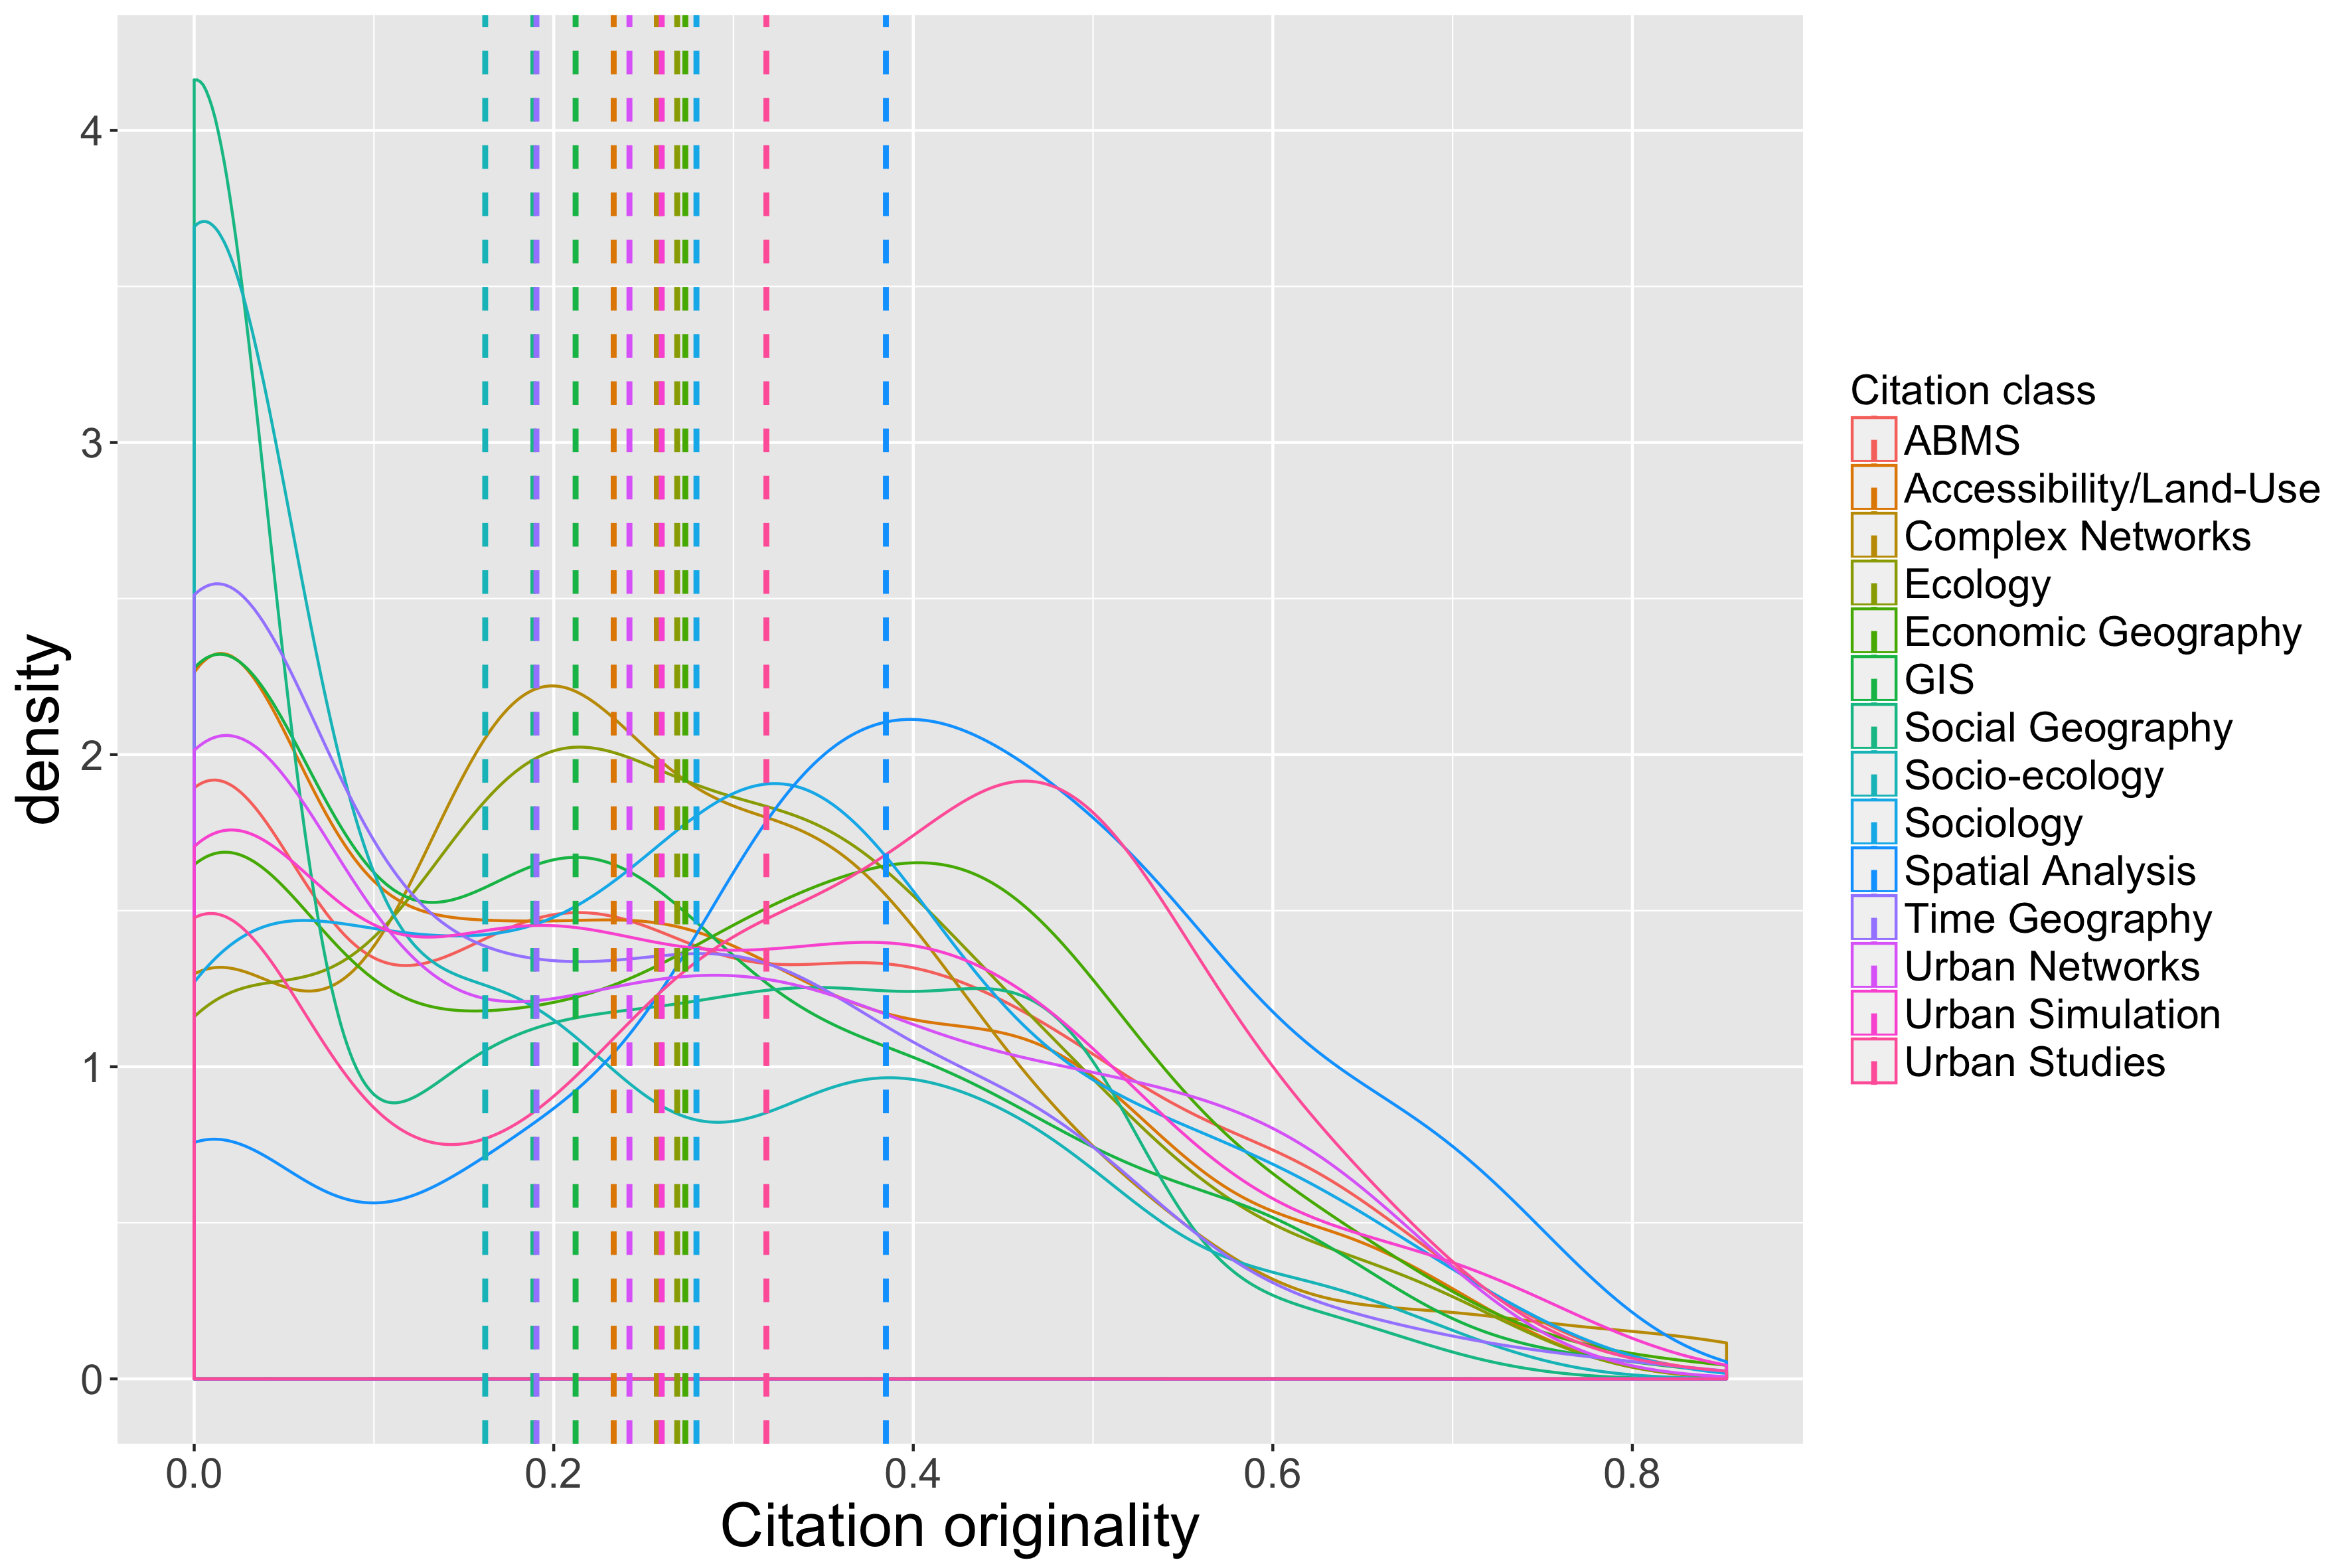
\includegraphics[width=0.8\linewidth]{figures/citation_originalities_citclass.png}
\end{center}

\footnotesize
\textit{Distribution of originalities (Herfindhal index) for how references are cited by different citation classes}

}

\sframe{Measuring interdisciplinarity}{



\begin{center}
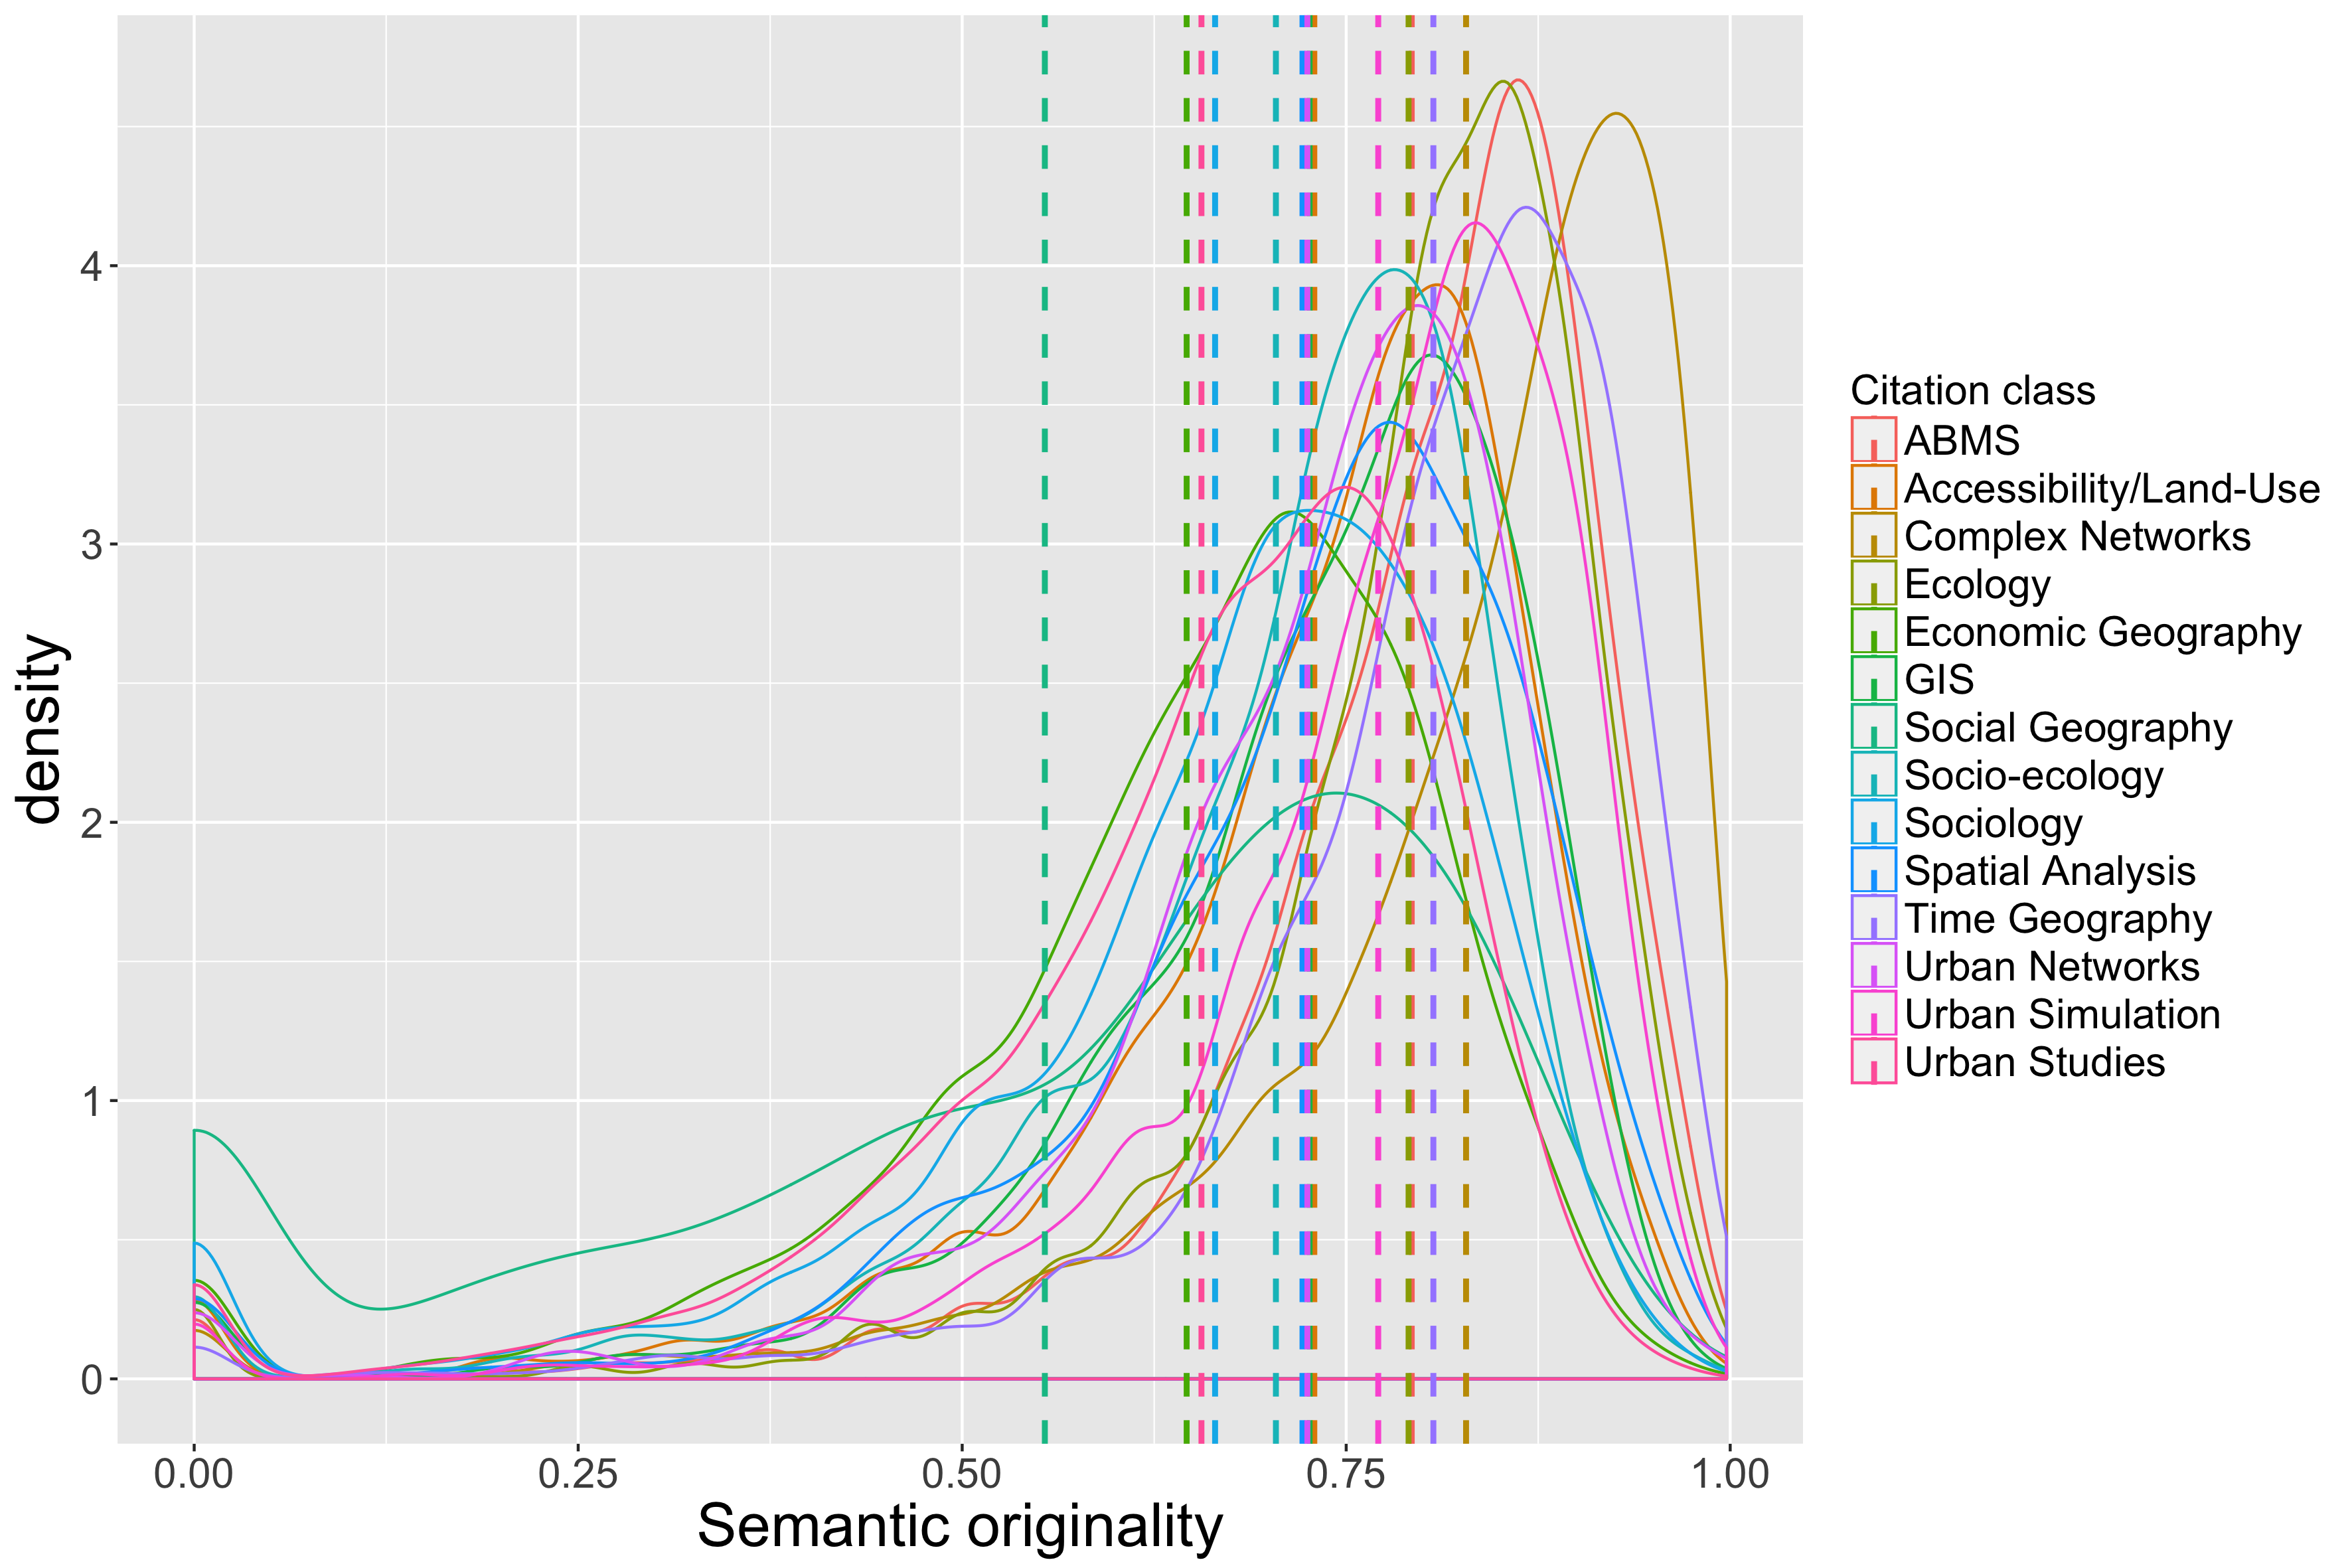
\includegraphics[width=0.8\linewidth]{figures/originalities_citclass.png}
\end{center}


\footnotesize
\textit{Distribution of semantic originalities}

}



\section{Discussion}

\sframe{Discussion}{

% We have this way shown the complementarity of classifications in the qualitative patterns they unveil, but also quantitatively in terms of interdisciplinarity measures and quantita- tively in terms of correlations. Our work can be extended regarding several aspects, of which we give some suggestions below.
%Developments
%A first development consists in the comparison of journals. The starting point for con- struction of the scientific environment, the journal Cybergeo, was the entry point but not the subject of our study. A development more focused on journals, trying for example to answer comparative issues, or to classify journals according to their effective level of inter- disciplinarity regarding different dimensions, would be potentially interesting. The collec- tion of precise data on the origin of references is however a first step that need to be solved first.
%The performance of the semantic classification was also not quantified here. A further validation of the relevance of using complementary information contained in both classifi- cations could be done by the analysis of modularities within the citation network, as done in Bergeaud et al. (2017). This would however require a baseline classification to compare with, which is not available in the type of data we use. Open repository such as arXiv (for physics mainly) or Repec (for Economics) provide API to access metadata including abstracts, and could be starting points for such targeted case studies.
%An other aspect on which our work could shed an interesting light is the univocity of scientific keywords between disciplines. Indeed, the same word can relate to different con- cepts in different disciplines. Co-occurrences patterns of specific words within the differ- ent citation communities should give information on the underlying concepts in each. For example, in the fields we studied, the word “model” will correspond to totally different concepts in Quantitative Geography and in Urbanism.

\justify

\textbf{Developments}

\medskip

$\rightarrow$ Journal dynamics and benchmarking, reflexivity for authors; fostering Open Science \cite{raimbault2019empowering}

\medskip

$\rightarrow$ Performance of the semantic classification for citation link prediction

\medskip

$\rightarrow$ Correspondence of terms between disciplines

\bigskip
\bigskip




% Applications
%A first potential application of our methodology relies on the facts that both classifications unveils thematic domains (objects of study), classical disciplines, methodological commu- nities. These different types of communities can indeed be understood as different Knowl- edge Domains. Raimbault (2017) postulates co-evolving Knowledge Domains in every process of scientific knowledge production, that are Theoretical, Empirical, Modeling, Methodology, Tools and Data domains. Most of them are necessary for any process, and investigations within one conditions the advances in others. A refinement of classifications, associated with supervised classification to associate knowledge domains to some com- munities (potentially using full texts to have more precise information on the proportion of each knowledge domains involved in each), would allow to quantify relations between domains. Furthermore, using temporal data with the date of publications, would yield an effective quantification of the co-evolution of domains in the sense of patterns of temporal correlations (e.g. Granger causality).
%Our work furthermore suggests that the different types of communities each unveil a different structure of science. This has implications for the construction of science maps, which refinement may go towards different maps for each dimension (which can more or less be associated to Knowledge Domains). Wen et al. (2017) have for example introduced such specific complementary maps as a new method of “bibliometric trian- gulation” in the case of water research.
%An other interesting direction is the application of our classifications to the quanti- fication of spatial diffusion of knowledge, as Maisonobe (2013) does for the diffusion of a specific question in molecular biology. It is not clear if different dimensions of knowledge diffuse the same way: for example citation practices can be correlated to social networks and thus exhibit different patterns than effective research contents. This phenomenon is suggested in terms of a co-evolution for semantics and social networks by Roth and Cointet (2010). Therefore, our work would allow to study such questions from complementary point of views.

\textbf{Applications}

\medskip

$\rightarrow$ Quantification of Domains of Knowledge \cite{raimbault2017applied}

\medskip

$\rightarrow$ Complementary dimensions in the structure of science

\medskip

$\rightarrow$ Spatial diffusion of knowledge \cite{doi:10.1162isala00283} 


% Positioning
% We finally discuss the positioning of our paper. The analysis developed did not pretend to construct maps of a given discipline, but indeed to allow authors and readers of the journal to better situate their work in their scientific neighborhood. As our approach is fully reproducible and does not require access to restricted databases, we argue that our contribution could foster open science and reflexivity. We therefore believe the tool we developed can contribute to an increased empower- ment of authors and to the development of open science practices. Among the various visions of Open Science (Fecher and Friesike 2014), the opening of data is always an important aspect, together with a development of reflexivity in all disciplines, beyond the sole Social Sciences to which it is classically associated. The first point is dealt with by our open tools for dataset construction, whereas the second is implied by the knowledge of the different dimensions of the scientific environment we studied, allowed by the multilayer methodology introduced. Using other dimensions and methodologies, Banos et al. (2018) illustrate this approach through an interactive application to analyse the corpus of the Cybergeo journal.


}








\sframe{Conclusion}{

% We have introduced a multi-dimensional approach to the understanding of interdiscipli- narity, based on citation network and semantic network analysis. Starting from a gen- eralist journal in Geography, we construct a large corpus of the citation neighborhood, from which we extract relevant keywords to elaborate a semantic classification. We then show qualitatively and quantitatively the complementarity of classifications. The meth- odology and associated tools are open and can be reused in similar studies for which data is difficult to access or poorly referenced in classical databases.

$\rightarrow$ A multi-dimensional approach to understand patterns of interdisciplinarity

\bigskip

$\rightarrow$ Open tools and methodology to foster Open Science


\bigskip
\bigskip

\textbf{Paper at} \url{https://doi.org/10.1007/s11192-019-03090-3}

(open version at \url{https://arxiv.org/abs/1712.00805})

\bigskip

\textbf{Open repositories for the paper and library}

\url{https://github.com/JusteRaimbault/HyperNetwork}

\url{https://github.com/JusteRaimbault/BiblioData}


\bigskip

\textbf{Data at} \texttt{http://dx.doi.org/10.7910/DVN/VU2XKT}

}



%%%%%%%%%%%%%%%%%%%%%
\begin{frame}[allowframebreaks]
\frametitle{References}
\bibliographystyle{apalike}
\bibliography{biblio}
\end{frame}
%%%%%%%%%%%%%%%%%%%%%%%%%%%%



%\sframe{Reserve slides}{
%
%\Huge
%
%\centering
%
%Reserve slides
%
%}



\end{document}

